\documentclass{template/openetcs_report}
% Use the option "nocc" if the document is not licensed under Creative Commons
%\documentclass[nocc]{template/openetcs_article}
\usepackage{rotating,url,color}
%\usepackage[hidelinks]{hyperref}
%hidelinks put some problems on some distributions
\usepackage{hyperref}
\graphicspath{{./template/}{.}{./images/}}
\begin{document}
\frontmatter
\project{openETCS}

%Please do not change anything above this line
%============================
% The document metadata is defined below

%assign a report number here
\reportnum{OETCS/WP7/O7.2.1~--~00/05}

%define your workpackage here
\wp{Work-Package 7: ``Secondary tools - Verification and Validation ''}

%set a title here
\title{Evaluation of supporting tools and methods against the WP2 requirements and task 1}

%set a subtitle here
\subtitle{Means and tools for Verification and Validation}

%set the date of the report here
\date{October 2013}

%define a list of authors and their affiliation here

\author{Marielle Petit-Doche}
\affiliation{Systerel}


\author{all participants of the benchmark}
\affiliation{WP7 partners}


\author{all participants of VnV  and Safety process}
\affiliation{WP4 partners}


% define the coverart
\coverart[width=350pt]{openETCS_EUPL.png}
 
%define the type of report
\reporttype{Evaluation}


\begin{abstract}
This document gives elements to evaluate the tools and methods to complete the primary toolchain and to support verification and validation activities, safety activities, moodel transformation and data management for the whole project.
 Evaluation on the means and tools of benchmark is also described.

\end{abstract}

%=============================
%Do not change the next three lines
\maketitle
\tableofcontents
\listoffiguresandtables
\newpage
%=============================


\begin{tabular}{|p{4.4cm}|p{8.7cm}|}
\hline
\multicolumn{2}{|c|}{Document information} \\
\hline
Work Package &  WP7  \\
Deliverable ID or doc. ref. & O7.2.1\\
\hline
Document title & Evaluation of supporting tools and methods against the WP2 requirements and task 1 - Vnv \\
Document version & 00.05 \\
Document authors (org.)  & Marielle Petit-Doche (Systerel)  \\
\hline
\end{tabular}

\begin{tabular}{|p{4.4cm}|p{8.7cm}|}
\hline
\multicolumn{2}{|c|}{Review information} \\
\hline
Last version reviewed & 00.04 \\
\hline
Main reviewers &  \\
 
\hline
\end{tabular}

\begin{tabular}{|p{2.2cm}|p{4cm}|p{4cm}|p{2cm}|}
\hline
\multicolumn{4}{|c|}{Approbation} \\
\hline
  &  Name & Role & Date   \\
\hline  
Written by    &  Marielle Petit-Doche & WP7-T7.1 Sub-Task Leader  & \\
\hline
Approved by & Michael Jastram & WP7 leader & \\
\hline
\end{tabular}

\begin{tabular}{|p{2.2cm}|p{2cm}|p{3cm}|p{5cm}|}
\hline
\multicolumn{4}{|c|}{Document evolution} \\
\hline
Version &  Date & Author(s) & Justification  \\
\hline  
00.01 & 19/07/2013 & M. Petit-Doche &  Document creation  \\
00.02 & 09/09/2013 & M. Petit-Doche &  Major evolutions in all document  \\
00.03 & 19/09/2013 & M. Petit-Doche &  Issues: 167, 168, 170  \\
00.04 & 23/09/2013 & M. Petit-Doche &  Issues: 164, 169, 174, 175, 177, 178  \\
00.05 & 01/10/2013 & M. Petit-Doche &  Split of document O7.2.1. Verification and Validation part \\
00.06 & 18/10/2013 & M. Petit-Doche &  Issues: 174, 178, 167\\
00.07 & 08/11/2013 & M. Petit-Doche &  Issues: 177, 179, 176, 180 \\
\hline  
\end{tabular}

% The actual document starts below this line
%=============================


%%%%%%%%%%%%%%%%%%%%%%%%%%%%%%%%%%%%%%%%%%%%%%%%%%%%%%%%%%%%%%
%%%              My macros (=> Sylvain Baro)               %%%
%%%%%%%%%%%%%%%%%%%%%%%%%%%%%%%%%%%%%%%%%%%%%%%%%%%%%%%%%%%%%%
\newcommand{\tbd}{\colorbox{cyan}{\%\%To Be Defined\%\%}}
\newcommand{\tbc}{\colorbox{cyan}{\%\%To Be Confirmed\%\%}}
\newcommand{\todo}[1]{\colorbox{cyan}{\%\%{#1}\%\%}}
\newlength{\origindent}

\newenvironment{issue}{
        \begin{quote}
        \begin{itshape}Open Issue.
}{
        \end{itshape}
        \end{quote}
}

\newenvironment{comment}{
        \begin{quote}
        \begin{itshape}Comment.
}{
        \end{itshape}
        \end{quote}
}

\newenvironment{justif}{
        \begin{quote}
        \begin{itshape}Justification.
}{
        \end{itshape}
        \end{quote}
}


\newenvironment{author_comment}{
        \begin{quote}
        \begin{itshape}\textcolor{green}{Author:}
}{
        \end{itshape}
        \end{quote}
}


\newenvironment{assessor1}{
        \begin{quote}
        \begin{itshape} \textcolor{blue}{Assessor 1:}
}{
        \end{itshape}
        \end{quote}
}


\newenvironment{assessor2}{
        \begin{quote}
        \begin{itshape}\textcolor{magenta}{Assessor 2:}
}{
        \end{itshape}
        \end{quote}
}

% Start here

\mainmatter



%-----------------------
\section{Motivation}
%-----------------------

%-----------------------
\section{Scope of the document}
%-----------------------

%----------------------
 \section{Reference documents}
%----------------------- 
\begingroup
%\renewcommand{\section}[2]{}%
\renewcommand{\chapter}[2]{}% for other classes
  \bibliographystyle{plain}
  \bibliography{wp7_bibliography}
\endgroup
%%% Local Variables: 
%%% mode: latex
%%% TeX-master: WP7-Toolchain_architecture"
%%% End: 


\chapter{Template}
\label{sec:template}

\section{Instructions}

\begin{description}
\item[\textcolor{green}{Author}] Author of the approaches description  \todo{Name -  Company}
\item[\textcolor{blue}{Assessor 1}] First assessor of the approaches \todo{Name - Company}
\item[\textcolor{magenta}{Assessor 2}] Second assessor of the approaches \todo{Name - Company}
\end{description}

In the sequel, main text is under the responsibilities of the author.

\begin{author_comment}
Author can add comments using this format at any place.
\end{author_comment}

\begin{assessor1}
First assessor can add comments using this format at any place.
\end{assessor1}

\begin{assessor2}
Second assessor can add comments using this format at any place.
\end{assessor2}

When a note is required, please follow this list :
\begin{description}
\item[0] not recommended, not adapted, rejected
\item[1] weakly recommended, adapted after major improvements, weakly rejected
\item[2] recommended, adapted (with light improvements if necessary)  weakly accepted
\item[3] highly recommended, well adapted,strongly accepted
\item[*] difficult to evaluate with a note (please add a comment under the table)
\end{description}

All the notes can be commented under each table.

\section{Presentation}

This section gives a quick presentation of the approach and the tool.

\begin{description}
\item[Name] \todo{Name of the approach and the tool}
\item[Web site] \todo{if available, how to  find information}
\item[Licence] \todo{Kind of licence}
\end{description}

\paragraph{Abstract} Short abstract on the approach and tool (10 lines max)

\paragraph{Publications} Short list of publications on the approach (5 max)


\section{Common criteria on secondary means and tools}
\label{common}
This section discusses the common criteria of the means and tools according to the project requirements on tools and the results of T7.1.

\subsection{Project and WP2 requirements}

The objectives of this list of criteria is to check if the proposed means and tools meet the main criteria of the project: open-source approaches, usability, modularity, coverage of the objectives,...

According WP2 requirements, give a note for characteristics of the use of the tool (from 0 to 3) :

\begin{tabular}{|l | c | c | c | c|}
\hline
& \textcolor{green}{Author} & \textcolor{blue}{Assessor 1} & \textcolor{magenta}{Assessor 2} & Total \\
\hline 
Open Source (D2.6-02-074) & & & &  \\
\hline 
Portability to operating systems (D2.6-02-075) & & & &  \\
\hline
Cooperation of tools (D2.6-02-076) & & & &  \\
\hline
Robustness (D2.6-02-078) & & & & \\
\hline
Modularity (D2.6-02-078.1) & & & & \\
\hline
Documentation management (D2.6-02-078.02) & & & & \\
\hline
Distributed software development (D2.6-02-078.03)  & & & & \\
\hline
Simultaneous multi-users (D2.6-02-078.04)   & & & & \\
\hline
Issue tracking (D2.6-02-078.05) & & & & \\
\hline
Differences between models (D2.6-02-078.06) & & & & \\
\hline
Version management (D2.6-02-078.07) & & & & \\
\hline
Concurrent version development (D2.6-02-078.08) & & & & \\
\hline
Model-based version control (D2.6-02-078.09) & & & & \\
\hline
Role traceability (D2.6-02-078.10) & & & & \\
\hline
Safety version traceability (D2.6-02-078.11) & & & & \\
\hline
Model traceability (D2.6-02-079) & & & & \\
\hline
Tool chain integration & & & & \\
\hline
Scalability & & & & \\
\hline
User Friendliness & & & & \\
\hline
\end{tabular}



\subsection{Qualification}

This section discusses how the tool can be classified according EN50128 requirements (D2.6-02-085). Some qualification shall be mandatory  if the tool is involved to design a SIL4 software.


\begin{tabular}{|l | c | c | c | c|}
\hline
& \textcolor{green}{Author} & \textcolor{blue}{Assessor 1} & \textcolor{magenta}{Assessor 2} & Total \\
\hline 
Tool manual (D.2.6-01-42.02) & & & &  \\
\hline
Proof of correctness (D.2.6-01-42.03)   & & & & \\
\hline
Existing industrial  usage  & & & & \\
\hline
Model verification & & & & \\
\hline
Test generation & & & & \\
\hline
Simulation, execution, debugging & & & & \\
\hline
Formal proof & & & & \\
\hline
\end{tabular}


Which level of tool qualification has been reached or will be reached within the next year ?


Score :
\begin{description}
\item[3] already qualified for this level
\item[2] qualification possible to this level, but some elements shall be provided
\item[0] qualification not recommended for this level
\end{description}


\begin{tabular}{|l | c | c | c | c|}
\hline
& \textcolor{green}{Author} & \textcolor{blue}{Assessor 1} & \textcolor{magenta}{Assessor 2} & Total \\
\hline 
class T1 & & & &  \\
\hline
class T2   & & & & \\
\hline
class T3  & & & & \\
\hline
\end{tabular}

\paragraph{Other elements for tool certification}


\subsection{Complementarity with primary toolchain}

The objectives of this list of criteria is to check if the proposed means and tools can be easily integrated to the primary toolchain.

\subsubsection{Language}


According to the decisions and the propositions of T7.1, how the mean and approach can be adapted to or can complete the chosen language and methods:

\begin{tabular}{|l | c | c | c | c|}
\hline
& \textcolor{green}{Author} & \textcolor{blue}{Assessor 1} & \textcolor{magenta}{Assessor 2} & Total \\
\hline 
SysML  & & & & \\
\hline
Scade method & & & & \\
\hline
EFS language & & & & \\
\hline
B Method & & & & \\
\hline
C language & & & & \\
\hline
\end{tabular}

\paragraph{SysML}
How the means or tools can complete SysML ?


\paragraph{Scade, EFS, Classical B}
How the means or tools can complete the current proposals for formal modeling language ?

\paragraph{C language}
How the means or tools can complete or be adapted to SIL4 software in C language ?

\subsubsection{Tools and platforms}

According to the decisions and the propositions of T7.1, how the mean and approach can be integrated to or can complete the chosen tools and platforms:

\begin{tabular}{|l | c | c | c | c|}
\hline
& \textcolor{green}{Author} & \textcolor{blue}{Assessor 1} & \textcolor{magenta}{Assessor 2} & Total \\
\hline 
Eclipse & & & &  \\
\hline
Papyrus  & & & & \\
\hline
Scade & & & & \\
\hline
EFS tools & & & & \\
\hline
B tools & & & & \\
\hline
\end{tabular}


\paragraph{Eclipse}
How the means or tools can be integrated to the Eclipse platform ?

\paragraph{Papyrus}
How the means or tools can complete  Papyrus ?


\paragraph{Scade, EFS, Classical B}
How the means or tools can complete the current proposals for formal modeling tools ?


\section{Means and tools for safety activities support}
\label{sec:safety}


This section defines the criteria for the means and tools dedicated to support of safety activities, in the WP4 workpackage. 

Criteria of this section are defined according \citep{D4.2.a}.

\subsection{Safety activities}

Which safety design activities are covered by the mean or tool (see \citep{D4.2.a} section 1.2) ?

\begin{tabular}{|l | c | c | c | c|}
\hline
& \textcolor{green}{Author} & \textcolor{blue}{Assessor 1} & \textcolor{magenta}{Assessor 2} & Total \\
\hline 
Preliminary Hazard Analysis & & & &  \\
\hline
System Hazard and Risk Analysis & & & & \\
\hline
Risk Assessment & & & & \\
\hline
Specification of System Safety Requirements & & & &  \\
\hline
Define Safety Related Functional Requirements & & & & \\
\hline
Specify Sub-System and Component & & & & \\
Safety requirements & & & & \\
\hline
Verify System, Sub-System and Component & & & &  \\
Safety requirements & & & &  \\
\hline
Validate System Safety Requirements & & & & \\
\hline
Establish Safety Case & & & & \\
\hline
\end{tabular}


\subsection{Input Artifacts}

Which artifacts are used as input of the mean or tool (see \citep{D4.2.a} section 1.4) ? 


\begin{tabular}{|l | c | c | c | c|}
\hline
& \textcolor{green}{Author} & \textcolor{blue}{Assessor 1} & \textcolor{magenta}{Assessor 2} & Total \\
\hline 
Safety Requirement & & & &  \\
\hline
Hazard log & & & & \\
\hline
Safety Case & & & & \\
\hline
\end{tabular}



\subsection{Output Artifacts}

Which artifacts are used as output of the mean or tool (see \citep{D4.2.a} section 1.4) ? 


\begin{tabular}{|l | c | c | c | c|}
\hline
& \textcolor{green}{Author} & \textcolor{blue}{Assessor 1} & \textcolor{magenta}{Assessor 2} & Total \\
\hline 
Safety Requirement & & & &  \\
\hline
Hazard log & & & & \\
\hline
Safety Case & & & & \\
\hline
\end{tabular}

\subsection{Expressiveness}


Which degree of formalisation is given to the artifacts by mean or tools (see \citep{D4.2.a} section 1.4) ? 


\begin{tabular}{|l | c | c | c | c|}
\hline
& \textcolor{green}{Author} & \textcolor{blue}{Assessor 1} & \textcolor{magenta}{Assessor 2} & Total \\
\hline 
Informal & & & &  \\
\hline
Semi-Formal & & & & \\
\hline
Formal & & & & \\
\hline
\end{tabular}


\subsection{Other criteria}
According to \citep{D4.2.a} section 2.2, provide some complement on the mean or tool:


\begin{tabular}{|l | c | c | c | c|}
\hline
& \textcolor{green}{Author} & \textcolor{blue}{Assessor 1} & \textcolor{magenta}{Assessor 2} & Total \\
\hline 
Top-Down approach  & & & &  \\
\hline
Bottom-up approach & & & & \\
\hline
Database capability & & & & \\
\hline
Database query ability & & & & \\
\hline
Safety requirement VnV & & & & \\
\hline
Traceability & & & & \\
\hline
Generation of documentation & & & & \\
\hline
\end{tabular}


\section{Other comments}



\begin{comment}
This section is available for the author or the assessors to  complete the description and criteria.
\end{comment}






\section{T7.1 Conclusion}


\begin{frame}{T7.1 Proposition}



\begin{itemize}
\item More than a year for the evaluation (1/3 of project duration)
\item Now at the middle term of the project
\item Two decision meetings with votes
\item Few activities mentioned as follow-up of the meetings
\item Next steps started in the project (WP7, WP3, WP4,...)
\item Few resources available
\end{itemize}

  \pause
  \textcolor{red}{Can we consider officially this task achieved ?}

\end{frame}



\appendix

\chapter{SCADE}

\begin{description}
\item[\textcolor{green}{Author}] Author of the approaches description  Uwe Steinke (Siemens)
\item[\textcolor{blue}{Assessor 1}] First assessor of the approaches David Mentré (MERCE)
\item[\textcolor{magenta}{Assessor 2}] Second assessor of the approaches Cécile Braunstein (Uni. Bremen)
\end{description}

In the sequel, main text is under the responsibilities of the author.

\begin{author_comment}
Author can add comments using this format at any place.
\end{author_comment}

\begin{assessor1}
First assessor can add comments using this format at any place.
\end{assessor1}

\begin{assessor2}
Second assessor can add comments using this format at any place.
\end{assessor2}

When a note is required, please follow this list :
\begin{description}
\item[0] not recommended, not adapted, rejected
\item[1] weakly recommended, adapted after major improvements, weakly rejected
\item[2] recommended, adapted (with light improvements if necessary)  weakly accepted
\item[3] highly recommended, well adapted,strongly accepted
\item[*] difficult to evaluate with a note (please add a comment under the table)
\end{description}

All the notes can be commented under each table.

\section{Presentation}

This section gives a quick presentation of the approach and the tool.

\begin{description}
\item[Name:] SCADE Suite / SCADE System / SCADE LifeCycle
\item[Web site: ] \url{http://esterel-technologies.com }
\item[Licence: ] Commercial
\end{description}

\paragraph{Abstract} Short abstract on the approach and tool (10 lines max)

SCADE is a formal modelling language targeted for safety-critical embedded control applications
in the avionics, rail, automotive and industrial automation domain. SCADE source code can be
written as text (for anyone who likes writing plain text) or (more usual) as schematic diagrams.

SCADE models are synchronously clocked data flow and state machines, that can be nested
and intermixed with each other without limitations. SCADE provides DO-178B- and EN50128-
certified code generators producing C or ADA code as output. SCADE models are therefore concrete, deterministic, executable and verifiable; it allows the production of rapid prototype as
well as of safety related target system software.

SCADE comes with an integrated development environment (SCADE Suite IDE) including
code generator, graphical simulator, model checker/prover, model test coverage analyzer, report
generators, version and requirements management gateway with interfaces to various other tools
like static code and timing analyzers, System/SysML modelling tools etc.. The IDE provides
automatization interfaces to be controlled from external tools, and all SCADE tools itself can
also be used in batch mode. In addition, plugins for Eclipse integration are available.

The SCADE paradigm of synchronously clocked data flow and state machines works perfect for
embedded control or industry automation software. It is less suitable for tasks like text processing
or computer graphic applications. SCADE models do not only describe the structure of software;
instead, they are the software implementation itself too. System architectures typically require a
higher abstraction means of description at top level like SysML. While SysML modelling can
be achieved with any SysML tools, SCADE System provides an automatic transformation from
SysML to SCADE.

\paragraph{Publications} Short list of publications on the approach (5 max)

\begin{itemize}
	\item \url{http://www.interested-ip.eu/}
  \item \url{http://http://www.interested-ip.eu/final-report.html/}

\end{itemize}

\section{Main usage of the approach}
\label{main_usage}
This section discusses the main usage of the approach.

According to the figure \ref{fig:main_process}, for which phases do you recommend the approach (give a note from 0 to  3) :

\begin{tabular}{|l | c | c | c | c|}
\hline
& \textcolor{green}{Author} & \textcolor{blue}{Assessor 1} & \textcolor{magenta}{Assessor 2} & Total \\
\hline 
System Analysis & 1      & 1     &1 & 3     \\
\hline
Sub-system  formal  design &  3 & 3     &3 & \textcolor{red}{\textbf{9}} \\
\hline
Software design & 3      & 3     & 3     & \textcolor{red}{\textbf{9}} \\
\hline
Software code generation & 3     & 3     &3 & \textcolor{red}{\textbf{9}} \\
\hline
\end{tabular}

\begin{author_comment}
SCADE can be used for analyzing tasks on system level, especially to clarify complex system behaviour and functions by practical modelling, execution, simulation and test. For a higher abstraction level, this should be enhanced with system modelling languages as SysML.
\end{author_comment}
According to the figure \ref{fig:main_process}, for which type of activities do you recommend the approach (give a note from 0 to  3) :

\begin{tabular}{|l | c | c | c | c|}
\hline
& \textcolor{green}{Author} & \textcolor{blue}{Assessor 1} & \textcolor{magenta}{Assessor 2} & Total \\
\hline 
Documentation &  3  & 2     &3 & \textcolor{magenta}{8}  \\
\hline
Modeling &  3  & 3     &3 & \textcolor{red}{\textbf{9}} \\
\hline
Design &  3  & 3     &3 & \textcolor{red}{\textbf{9}} \\
\hline
Code generation &  3  & 3     &3 & \textcolor{red}{\textbf{9}} \\
\hline
Verification &  3  & 2     &3 & \textcolor{magenta}{8} \\
\hline
Validation &  3  & 2     &3 & \textcolor{magenta}{8} \\
\hline
Safety analyses &  0  & 1     & \textcolor{green}{0}   & 1     \\
\hline
\end{tabular}


\begin{assessor1}
Verification capabilities of SCADE Verifier are limited by state space
explosion. As far as I know, very few SCADE users are doing formal
verification except for very small designs.

The test facilities are however much used.
\end{assessor1}


\paragraph{Known usages} Have you some examples of usage of this approach to  compare with the OpenETCS objectives ?

Field of usage: Safety critical systems like
\begin{itemize}
	\item Rail interlocking systems
	\item Rail track vacancy detection systems
	\item Rail train control systems
	\item Rail Level-crossing protection systems
	\item Avionic flight controllers
\end{itemize}

\section{Language}
This section discusses the main element of the language.

Which are the main characteristics of the language :

\begin{tabular}{|l | c | c | c | c|}
\hline
& \textcolor{green}{Author} & \textcolor{blue}{Assessor 1} & \textcolor{magenta}{Assessor 2} & Total \\
\hline 
Informal language &  0  & \textcolor{green}{0} & \textcolor{green}{0}   &  0 \\
\hline 
Semi-formal language &  0  & 3     & \textcolor{green}{0}   &  3 \\
\hline
Formal language &  3  & 3     &3 &  \textcolor{red}{\textbf{9}} \\
\hline
Structured language &  3  & 3     &3 & \textcolor{red}{\textbf{9}} \\
\hline
Modular language &  3  & 2     &3 & \textcolor{magenta}{8} \\
\hline
Textual language & 3     & 3     &3 & \textcolor{red}{\textbf{9}} \\
\hline
Mathematical symbols or code & 3     & 3     &3 & \textcolor{red}{\textbf{9}} \\
\hline
Graphical language & 3     & 3     &3 & \textcolor{red}{\textbf{9}} \\
\hline
\end{tabular}

According WP2 requirements, give a note for the capabilities of the language (from 0 to 3) :

\begin{tabular}{|l | c | c | c | c|}
\hline
& \textcolor{green}{Author} & \textcolor{blue}{Assessor 1} & \textcolor{magenta}{Assessor 2} & Total \\
\hline
Declarative formalization of properties (D2.6-02-066) &
2  & 2     &2 & \textcolor{blue}{6} \\
\hline
Simple formalization of properties (D2.6-02-066.01) &
2 & 2     &2 & \textcolor{blue}{6} \\
\hline
Scalability : capability to design large model &  3
& 2     &3 & \textcolor{magenta}{8} \\
\hline
Easily translatable to other languages (D2.6-02-066) &
3  & 3     &3 & \textcolor{red}{\textbf{9}} \\
\hline
Executable directly (D2.6-02-071) & 3      & 3     &3 & \textcolor{red}{\textbf{9}} \\
\hline
Executable after translation to a code (D2.6-02-071) &
3& 3     &3 & \textcolor{red}{\textbf{9}} \\
(precise if the translation is automatic) &  3& 3     &3 & \textcolor{red}{\textbf{9}} \\
\hline
Simulation, animation (D2.6-02-071) &  3 & 3     &3 & \textcolor{red}{\textbf{9}} \\
\hline
Easily understandable (D2.6-02-065) &  3& 3     &3 & \textcolor{red}{\textbf{9}} \\
\hline
Expertise level needed (0 High level, 3 few level) &
2 & 2     &2 & \textcolor{blue}{6} \\
\hline
Standardization (D2.6-02-067) &  3& \textcolor{green}{0} &3 & \textcolor{blue}{6} \\
\hline
Documented (D2.6-02-067) &  3 & 2     &3 & \textcolor{magenta}{8} \\
\hline
Extensible language (D.2.6-01-28) &  2& 2     &1 & \textcolor{blue}{5} \\
\hline
\end{tabular}
\begin{author_comment}
SCADE is a strictly textual and graphical formal language. It allows to be extended with user-defined operators. Especially the graphical representation is easy to learn and understand; nevertheless the rich tool suite covering most aspects of a EN50128 compliant process causes an appropriate learning effort by amount.
\end{author_comment}


\begin{assessor1}
  I am still skeptical that graphical representation is the best way
  to represent big systems.

  SCADE language lacks some facilities, like library parametrization
  by parameters (like OCaml functor, C++ template or Ada generics).
\end{assessor1}

\paragraph{Documentation} Describe how the language is documented, the existing guidelines, coding rules, standardization...

SCADE provides a detailed documentation set:

\begin{itemize}
	\item Getting Started
	\item SCADE Language Tutorial
	\item SCADE Suite User Manual
	\item SCADE Suite Technical Manual
	\item SCADE Suite Libraries Manual
	\item SCADE Language Primer
	\item SCADE Language Reference Manual
	\item Gateway Guidelines for LabView, Rhapsody, Simulink
	\item RTOS Adaptor Guidelines
	\item Timing and Stack Analysis Tools
	\item SCADE LifeCycle Documentation
	\item SCADE Suite Metamodels
	\item SCADE Glossary
	\item ...
\end{itemize}


\paragraph{Language usage} Describe the possible restriction on the language. 
SCADE is less suitable for tasks like text processing or computer graphic applications.


\section{System Analysis}
This section discusses the usage of the approach for system analysis.
It can be skipped depending the results of \ref{main_usage}.

Acoording WP2 requirements, how the approach can be involved for the sub-system requirement specification ?

\begin{tabular}{|l | c | c | c | c|}
\hline
& \textcolor{green}{Author} & \textcolor{blue}{Assessor 1} & \textcolor{magenta}{Assessor 2} & Total \\
\hline
Independent System functions definition (D.2.6-X-10.1.1)  &
3& 3     &3 & \textcolor{red}{\textbf{9}}  \\
\hline 
System architecture design (D.2.6-X-10.1.2) & 1     & 1     &
0& 3      \\
\hline
System data flow identification (D2.6-02-045.02.3)  &
3& 2     &3 & \textcolor{magenta}{8} \\
\hline
Sub-system focus (D2.6-02-045.02.4)  &  2& 2     &2 &  \textcolor{blue}{6} \\
\hline
System interfaces definition (D2.6-02-045.02.5)  &
2& 3     &3 & \textcolor{magenta}{8}  \\
\hline
System requirement allocation (D2.6-02-045.03)  &  3&
1 &3 &  \textcolor{magenta}{7} \\
\hline
Traceability with SRS (D2.6-02-045.05)  &  3& 3     &3 & \textcolor{red}{\textbf{9}}  \\
\hline
Traceability with Safety activities (D2.6-02-046)  &
3 & 3     &3 & \textcolor{red}{\textbf{9}}  \\
\hline
\end{tabular}

\begin{author_comment}
Although SCADE is not made for system analysis, it can be used for the following aspects on system level: Modelling of (separate) system functions, data flows, state machines and interfaces. It provides an excellent tracebility support between many different kinds of documents and other tools.  
\end{author_comment}


\section{Sub-System formal design}
This section discusses the usage of the approach for sub-system formal design.
It can be skipped depending the results of \ref{main_usage}.

Two kinds of model can be planned during this phase: semi-formal models to  cover the SSRS (D2.6-02-047.01) and strictly formal  models to  focuss on some functional and safety aspects (D2.6-02-049).  Obviously some strictly  formal means can be used to define the semi-formal  model.

\subsection{Semi-formal model}

\begin{author_comment}
SCADE models are formal. Since the following table addresses many aspects that SCADE covers in a formal way it is filled anyway. But keep in mind: it's formal - instead of semi-formal.  
\end{author_comment}


Concerning formal model, how the WP2 requirements are covered ?

\begin{tabular}{|l | c | c | c | c|}
\hline
& \textcolor{green}{Author} & \textcolor{blue}{Assessor 1} & \textcolor{magenta}{Assessor 2} & Total \\
\hline 
Consistency to SSRS (D2.6-02-047.02) & 2     & 2     & & - \\
\hline
Coverage of SSRS (D2.6-02-047.02.01)  & 3     & 2     & & - \\
\hline
Coverage of SSHA (D2.6-02-047.02.02)  &  3& 3     & & - \\
\hline
Management of requirement justification (D2.6-02-047.02.03)  &
3& 3     & & - \\
\hline
Traceability to  SSRS (D2.6-02-047.02.05)  &  3& 3     & & - \\
\hline
Traceability of exported requirements (D2.6-02-047.02.06)  &
3& 3     & & - \\
\hline
Simulation or animation (D2.6-02-048 partial)  &  3&
3& & - \\
\hline
Execution (D2.6-02-048 partial)  & 3     & 3     & & - \\
\hline
Extensible to strictly formal model (D2.6-02-049.3) &
3  & 3     & & - \\
\hline
Easy to  refine towards strictly formal model (D2.6-02-049.4) &
3 & 3     & & - \\
\hline
Extensible and modular design (D2.6-02-050)  & 3     & 2     & & - \\
\hline
Extensible to software architecture and design (D2.6-02-068)   &
3& 3     & & - \\
\hline
\end{tabular}

Concerning safety properties management, how the WP2 requirements are covered ?

\begin{tabular}{|l | c | c | c | c|}
\hline
& \textcolor{green}{Author} & \textcolor{blue}{Assessor 1} & \textcolor{magenta}{Assessor 2} & Total \\
\hline 
Safety function isolation (D2.6-02-052)  &  2& 2     & & - \\
\hline 
Safety properties formalisation (D2.6-02-057)  &  2&
1 & & - \\
\hline
Logical expression (D2.6-02-066.02.01)  &  3& 3     & & - \\
\hline
Timing constraints (D2.6-02-066.02.02)  &  2 & 2     & & - \\
\hline
Safety properties validation (D2.6-02-058.02)  &  2& 2     & & - \\
\hline
Logical properties assertion (D2.6-02-072)  &  2& 2     & & - \\
\hline
Check  of assertions (D2.6-02-072.1)  &  2& 2     & & - \\
\hline
\end{tabular}

\begin{author_comment}
SCADE is a modelling language for functions. Therefore, only the functional aspects of properties are addressed.  
\end{author_comment}


\begin{assessor1}
  SCADE lacks facilities to check for example data flow properties
  (inputs, outputs, in-outs) of a function.
\end{assessor1}


Does the language allow to  formalize (D2.6-02-069):

\begin{tabular}{|l | c | c | c | c|}
\hline
& \textcolor{green}{Author} & \textcolor{blue}{Assessor 1} & \textcolor{magenta}{Assessor 2} & Total \\
\hline 
State machines  & 3     & 3     & & - \\
\hline
Time-outs  & 3     & 3     & & - \\
\hline
Truth tables  & 3     & 3     & & - \\
\hline
Arithmetic  & 3     & 3     & & - \\
\hline
Braking curves  & 3     & 3     & & - \\
\hline
Logical statements & 3     & 3     & & - \\
\hline
Message and fields & 2     & 2     & & - \\
\hline
\end{tabular}

\paragraph{Additional comments on semi-formal  model} Do you think your semi-formal  model is sufficient to cover a safe design of the on-board unit until code generation ?
All comments on links to  other models, validation and verification activities are welcomed.

\begin{author_comment}
SCADE is targeted for these purposes.   
\end{author_comment}


\subsection{Strictly formal model}

Concerning strictly formal model, how the WP2 requirements are covered ?

\begin{tabular}{|l | c | c | c | c|}
\hline
& \textcolor{green}{Author} & \textcolor{blue}{Assessor 1} & \textcolor{magenta}{Assessor 2} & Total \\
\hline 
Consistency to SFM (D2.6-02-049.2) & 3     & 3     &3 & \textcolor{red}{\textbf{9}} \\
\hline
Coverage of SSRS (D2.6-02-049.2)  &3 & 3     &3 &  \textcolor{red}{\textbf{9}}  \\
\hline
Traceability to  SSRS (D2.6-02-049.3)  &3 & 3     &3 & \textcolor{red}{\textbf{9}}  \\
\hline
Extensible to software design (D2.6-02-051)  &3 & 3     &3 & \textcolor{red}{\textbf{9}}  \\
\hline
Safety function isolation (D2.6-02-052)  &  3& 2     &3 & \textcolor{magenta}{8}  \\
\hline 
Safety properties formalisation (D2.6-02-057)  &  2&
2&2 & \textcolor{blue}{6}  \\
\hline
Logical expression (D2.6-02-066.02.01)  &  3&3 &3 & \textcolor{red}{\textbf{9}}  \\
\hline
Timing constraints (D2.6-02-066.02.02)  &  3&2 &3 & \textcolor{magenta}{8} \\
\hline
Safety properties validation (D2.6-02-058.03)  &  2& 2     &2 & \textcolor{blue}{6}  \\
\hline
Logical properties assertion (D2.6-02-072)  &  2& 2     &2 & \textcolor{blue}{6} \\
\hline
Proof of assertions (D2.6-02-072.2)  &  2 & 2     &3 & \textcolor{magenta}{7} \\
\hline
\end{tabular}

Does the language allow to  formalize (D2.6-02-070):

\begin{tabular}{|l | c | c | c | c|}
\hline
& \textcolor{green}{Author} & \textcolor{blue}{Assessor 1} & \textcolor{magenta}{Assessor 2} & Total \\
\hline 
State machines  & 3     & 3     &3 & \textcolor{red}{\textbf{9}} \\
\hline
Time-outs  & 3     & 2     &3 & \textcolor{magenta}{8} \\
\hline
Truth tables  & 3     & 3     &3 & \textcolor{red}{\textbf{9}} \\
\hline
Arithmetic  & 3    & 3     &3 & \textcolor{red}{\textbf{9}} \\
\hline
Braking curves  & 3    & 3     &3 & \textcolor{red}{\textbf{9}} \\
\hline
Logical statements & 3    & 3     &3 & \textcolor{red}{\textbf{9}} \\
\hline
Message and fields &3 & 2     &3 & \textcolor{magenta}{8} \\
\hline
\end{tabular}

\paragraph{Additional comments on semi-formal  model} Do you think your strictly formal  model can be directly defined from the SSRS ?
All comments on links to  other models, validation and verification activities are welcomed.

\begin{author_comment}
SCADE is targeted for these purposes.   
\end{author_comment}
\begin{assessor2}
A SCADE model my be directly defined from the SSRS, this implies that
code may directly be generated from the SSRS.
\end{assessor2}


\section{Software design}
This section discusses the usage of the approach for software design.
It can be skipped depending the results of \ref{main_usage}.

\subsection{Functional design}

How the approach allows to  produce a functional software model of the on-board unit ?

\begin{tabular}{|l | c | c | c | c|}
\hline
& \textcolor{green}{Author} & \textcolor{blue}{Assessor 1} & \textcolor{magenta}{Assessor 2} & Total \\
\hline
Derivation from system semi-formal model  & 3     & 3     &3 & \textcolor{red}{\textbf{9}} \\
\hline 
Software architecture description  & 3     & 3     &3 & \textcolor{red}{\textbf{9}} \\
\hline
Software constraints  & 3     & 2     &3 & \textcolor{magenta}{8} \\
\hline
Traceability  & 3     & 3     &3 & \textcolor{red}{\textbf{9}} \\
\hline
Executable  & 3     & 3     &3 & \textcolor{red}{\textbf{9}} \\
\hline
\end{tabular}

\subsection{SSIL4 design}

How the approach allows to  produce in safety a software model ?

\begin{tabular}{|l | c | c | c | c|}
\hline
& \textcolor{green}{Author} & \textcolor{blue}{Assessor 1} & \textcolor{magenta}{Assessor 2} & Total \\
\hline
Derivation from system semi-formal or strictly formal model  &
3 & 3     &3 & \textcolor{red}{\textbf{9}} \\
\hline 
Software architecture description  & 3     & 3     &3 & \textcolor{red}{\textbf{9}} \\
\hline
Software constraints  & 3     & 3     &3 & \textcolor{red}{\textbf{9}} \\
\hline
Traceability  & 3     & 3     &3 & \textcolor{red}{\textbf{9}} \\
\hline
Executable  & 3     & 3     &3 & \textcolor{red}{\textbf{9}} \\
\hline
Conformance to EN50128 § 7.2  & 3     & 3     &3 & \textcolor{red}{\textbf{9}} \\
\hline
Conformance to EN50128 § 7.3  & 3     & 3     &3 & \textcolor{red}{\textbf{9}} \\
\hline
Conformance to EN50128 § 7.4  & 3    & 3     &3 & \textcolor{red}{\textbf{9}} \\
\hline
\end{tabular}

Which criteria for software architecture are covered by the methodology
(see EN50128 table A.3) :

\begin{tabular}{|l | c | c | c | c|}
\hline
& \textcolor{green}{Author} & \textcolor{blue}{Assessor 1} & \textcolor{magenta}{Assessor 2} & Total \\
\hline
Defensive programming  & 3    * & \textcolor{green}{0} &3 &  6 \\
\hline 
Fault detection \& diagnostic  & \textcolor{green}{0} * & \textcolor{green}{0} & \textcolor{green}{0}   & \textcolor{green}{0} \\
\hline
Error detecting code  & \textcolor{green}{0} * & \textcolor{green}{0} & \textcolor{green}{0}   & \textcolor{green}{0} \\
\hline
Failure assertion programming & 1     & \textcolor{green}{0} & \textcolor{green}{0}   & 1     \\
\hline
Diverse programming & \textcolor{green}{0} * & \textcolor{green}{0} & \textcolor{green}{0}   & \textcolor{green}{0} \\
\hline
Memorising executed cases & \textcolor{green}{0} * & 1     &2 & 3     \\
\hline
Software error effect analysis & \textcolor{green}{0} * & \textcolor{green}{0} & \textcolor{green}{0}   & \textcolor{green}{0} \\
\hline
Fully defined interface & 3     & 3     &3 & \textcolor{red}{\textbf{9}} \\
\hline
Modelling  & 3     & 3     &3 & \textcolor{red}{\textbf{9}} \\
\hline
Structured methodology & 3     & 3     &3 & \textcolor{red}{\textbf{9}} \\
\hline
\end{tabular}

\begin{author_comment}
The * are out of scope of SCADE. It does not support or prohibit these techniques in a specific way.   
\end{author_comment}


\section{Software code generation}
This section discusses the usage of the approach for software code generation.
It can be skipped depending the results of \ref{main_usage}.

Which criteria for software design and implementation are covered by the methodology
(see EN50128 table A.4) :

\begin{tabular}{|l | c | c | c | c|}
\hline
& \textcolor{green}{Author} & \textcolor{blue}{Assessor 1} & \textcolor{magenta}{Assessor 2} & Total \\
\hline
Formal methods  & 3     & 2     &3 & \textcolor{magenta}{8} \\
\hline 
Modeling  & 3     & 3     &3 & \textcolor{red}{\textbf{9}} \\
\hline
Modular approach (mandatory) & 3     & 3     &3 & \textcolor{red}{\textbf{9}} \\
\hline
Components & 3     & 3     &3 & \textcolor{red}{\textbf{9}} \\
\hline
Design and coding standards (mandatory) & 3     & 2     &3 & \textcolor{magenta}{8} \\
\hline
Strongly typed programming language & 3     & 3     &3 & \textcolor{red}{\textbf{9}} \\
\hline
\end{tabular}

\begin{assessor1}
  Does SCADE allow to check coding rules at diagram level? I don't
  think so.

  Set of properties and extent of their verification is limited in
  SCADE.
\end{assessor1}



\section{Main usage of the tool}
\label{main_usage}

This section discusses the main usage of the tool.

Which task are covered by the tool ?


\begin{tabular}{|l | c | c | c | c|}
\hline
& \textcolor{green}{Author} & \textcolor{blue}{Assessor 1} & \textcolor{magenta}{Assessor 2} & Total \\
\hline 
Modelling support & 3     & 3     &3 & \textcolor{red}{\textbf{9}} \\
\hline
Automatic translation  & 3     & 3     &3 & \textcolor{red}{\textbf{9}} \\
\hline
Code Generation  & 3     & 3     &3 & \textcolor{red}{\textbf{9}} \\
\hline
Model verification & 3     & 2     &2 & \textcolor{magenta}{7} \\
\hline
Test generation & 2     & 1     &1 & 4     \\
\hline
Simulation, execution, debugging & 3     & 3     &3 & \textcolor{red}{\textbf{9}} \\
\hline
Formal proof & 3     & 2     &2 & \textcolor{magenta}{7} \\
\hline
\end{tabular}

\paragraph{Modelling support}
Does the tool provide a  textual or a graphical editor ? 

\begin{itemize}
	\item Yes, both.
\end{itemize}


\paragraph{Automatic translation and code generation}
Which translation or code generation is supported by the tool ?

\begin{itemize}
	\item Validated translation of SCADE models into C or ADA code.
\end{itemize}

\paragraph{Model verification}
Which verification on models are provided by the tool?

\begin{itemize}
	\item Simulation
	\item animation
	\item verification via manual or script-based test suites
	\item Model test coverage for structural model coverage measurement
	\item Formal proving
\end{itemize}

\paragraph{Test generation}
Does the tool allow to generate tests ? For  which purpose ?

\begin{itemize}
	\item SCADE offers test suites to be built via test scripts
	\item For automatic model based test case generation tools like RT-Tester are applicable
\end{itemize}

\paragraph{Simulation, execution, debugging}
Does the tool allow to simulate or to debug step by step a model or a code ?

\begin{itemize}
	\item It allows simulation on a clock by clock base by executing the generated code while the model behaviour is visualized graphically
	\item Graphical model debugging with breakpoint capabilities
	\item Playback function for logfiles from the field
\end{itemize}

\paragraph{Formal proof}
Does the tool allow formal proof ?  How ?

\begin{itemize}
	\item SCADE integrates the Prover design verifier. 
	\item the provable properties have to be modelled with SCADE Suite and connected to the target model in an target-observer configuration
\end{itemize}


\begin{assessor1}
  Formal verification is limited by state space explosion.
\end{assessor1}

\section{Use of the tool}


According WP2 requirements, give a note for characteristics of the use of the tool (from 0 to 3) :

\begin{tabular}{|l | c | c | c | c|}
\hline
& \textcolor{green}{Author} & \textcolor{blue}{Assessor 1} & \textcolor{magenta}{Assessor 2} & Total \\
\hline 
Open Source (D2.6-02-074) &  0& \textcolor{green}{0} & \textcolor{green}{0}   & \textcolor{green}{0} \\
\hline 
Portability to operating systems (D2.6-02-075) &  3*&
1 & \textcolor{green}{0}   & 4     \\
\hline
Cooperation of tools (D2.6-02-076) &  3& 3     &2 & \textcolor{magenta}{8} \\
\hline
Robustness (D2.6-02-078) &  3& 3     &3 & \textcolor{red}{\textbf{9}} \\
\hline
Modularity (D2.6-02-078.1) &  3& 3     &3 & \textcolor{red}{\textbf{9}} \\
\hline
Documentation management (D2.6-02-078.02) &  3& 3     &3 & \textcolor{red}{\textbf{9}} \\
\hline
Distributed software development (D2.6-02-078.03)  &
2& 2     &2 & \textcolor{blue}{6} \\
\hline
Simultaneous multi-users (D2.6-02-078.04)   &  1& 1     &1 & 3     \\
\hline
Issue tracking (D2.6-02-078.05) &  0& \textcolor{green}{0}   & \textcolor{green}{0}   & \textcolor{green}{0} \\
\hline
Differences between models (D2.6-02-078.06) &  3& 3     &3 & \textcolor{red}{\textbf{9}} \\
\hline
Version management (D2.6-02-078.07) &  3& 3     &3 & \textcolor{red}{\textbf{9}} \\
\hline
Concurrent version development (D2.6-02-078.08) &  2&
2& * & 4    * \\
\hline
Model-based version control (D2.6-02-078.09) &  3& 3     &3 & \textcolor{red}{\textbf{9}} \\
\hline
Role traceability (D2.6-02-078.10) &  0& \textcolor{green}{0} & \textcolor{green}{0}   & \textcolor{green}{0} \\
\hline
Safety version traceability (D2.6-02-078.11) &  0& \textcolor{green}{0} & \textcolor{green}{0}   & \textcolor{green}{0} \\
\hline
Model traceability (D2.6-02-079) & 3     & 3     &3 & \textcolor{red}{\textbf{9}} \\
\hline
Tool chain integration & 3     & 3     &* & \textcolor{blue}{6} * \\
\hline
Scalability & 3     & 3     &3 & \textcolor{red}{\textbf{9}} \\
\hline
\end{tabular}

\begin{author_comment}
* The SCADE tool suite requires MS Windows. The generated executable code is able to run on any operating system and on platforms without an operation system.   
\end{author_comment}

\begin{assessor2}managment
SCADE is a almost complete tool chain. Missing multi-users and system design.
\end{assessor2}
\section{Certifiability}

This section discusses how the tool can be classified according EN50128 requirements (D2.6-02-085).

\begin{author_comment}
SCADE is targeted to be certifiable. Validation documentation is available.   
\end{author_comment}


\begin{tabular}{|l | c | c | c | c|}
\hline
& \textcolor{green}{Author} & \textcolor{blue}{Assessor 1} & \textcolor{magenta}{Assessor 2} & Total \\
\hline 
Tool manual (D.2.6-01-42.02) & 3     & 3     &3 & \textcolor{red}{\textbf{9}} \\
\hline
Proof of correctness (D.2.6-01-42.03)   & 3     & 3     &3 & \textcolor{red}{\textbf{9}} \\
\hline
Existing industrial  usage  & 3     & 3     &3 & \textcolor{red}{\textbf{9}} \\
\hline
Model verification & 3     & 2     &3 & \textcolor{magenta}{8} \\
\hline
Test generation & 2     & 2     &2 & \textcolor{blue}{6} \\
\hline
Simulation, execution, debugging & 3     & 3     &3 & \textcolor{red}{\textbf{9}} \\
\hline
Formal proof & 3     & 2     &2 & \textcolor{magenta}{7} \\
\hline
\end{tabular}

\paragraph{Other elements for tool certification}

\section{Other comments}
Please to  give free comments on the approach.




% LocalWords:  SCADE

\chapter{SystemC}
\label{sec:systemC}

\section{Instructions}

\begin{description}
\item[\textcolor{green}{Author}] Author of the approaches description  \todo{Name -  Company}
\item[\textcolor{blue}{Assessor 1}] First assessor of the approaches \todo{Name - Company}
\item[\textcolor{magenta}{Assessor 2}] Second assessor of the approaches \todo{Name - Company}
\end{description}

In the sequel, main text is under the responsibilities of the author.

\begin{author_comment}
Author can add comments using this format at any place.
\end{author_comment}

\begin{assessor1}
First assessor can add comments using this format at any place.
\end{assessor1}

\begin{assessor2}
Second assessor can add comments using this format at any place.
\end{assessor2}

When a note is required, please follow this list (inspired from Technology Readiness Level, see \url{http://en.wikipedia.org/wiki/Technology\_readiness\_level}) :

\begin{description}
\item[0] not recommended / rejected / no integration possible or valuable / not adapted for this topic / not available for this topic
\item[1] weakly recommended / adapted after major improvements / weakly rejected / concept of integration roughly defined / adapted after major improvements / available after major developments
\item[2] recommended / adapted (with light improvements if necessary)  weakly accepted / integration prototyped or defined in details / adapted after small improvements / available after small developments or tests
\item[3] highly recommended / well adapted / strongly accepted / integration done and tested / well adapted to the purpose / available and suitable for the purpose All the notes can be commented under each table.
\item[*] difficult to evaluate with a note (please add a comment under the table)
\end{description}


All the notes can be commented under each table.

This section defines the criteria for the means and tools dedicated to verification and validation activities, in the WP4 workpackage. 

Criteria of this section are defined according \citep{D4.1}.

\section{Presentation}

This section gives a quick presentation of the approach and the tool.

\begin{description}
\item[Name] \todo{Name of the approach and the tool}
\item[Web site] \todo{if available, how to  find information}
\item[Licence] \todo{Kind of licence}
\end{description}

\paragraph{Abstract} Short abstract on the approach and tool (10 lines max)

\paragraph{Publications} Short list of publications on the approach (5 max)


\section{Common criteria on secondary means and tools}
\label{common}
This section discusses the common criteria of the means and tools according to the project requirements on tools and the results of T7.1.

\subsection{Project and WP2 requirements}

The objectives of this list of criteria is to check if the proposed means and tools meet the main criteria of the project: open-source approaches, usability, modularity, coverage of the objectives,...

According WP2 requirements, give a note for characteristics of the use of the tool (from 0 to 3) :

\begin{tabular}{|l | c | c | c | c|}
\hline
& \textcolor{green}{Author} & \textcolor{blue}{Assessor 1} & \textcolor{magenta}{Assessor 2} & Total \\
\hline 
Open Source (D2.6-02-074) & & & &  \\
\hline 
Portability to operating systems (D2.6-02-075) & & & &  \\
\hline
Cooperation of tools (D2.6-02-076) & & & &  \\
\hline
Robustness (D2.6-02-078) & & & & \\
\hline
Modularity (D2.6-02-078.1) & & & & \\
\hline
Documentation management (D2.6-02-078.02) & & & & \\
\hline
Distributed software development (D2.6-02-078.03)  & & & & \\
\hline
Simultaneous multi-users (D2.6-02-078.04)   & & & & \\
\hline
Issue tracking (D2.6-02-078.05) & & & & \\
\hline
Differences between models (D2.6-02-078.06) & & & & \\
\hline
Version management (D2.6-02-078.07) & & & & \\
\hline
Concurrent version development (D2.6-02-078.08) & & & & \\
\hline
Model-based version control (D2.6-02-078.09) & & & & \\
\hline
Role traceability (D2.6-02-078.10) & & & & \\
\hline
Safety version traceability (D2.6-02-078.11) & & & & \\
\hline
Model traceability (D2.6-02-079) & & & & \\
\hline
Tool chain integration & & & & \\
\hline
Scalability & & & & \\
\hline
User Friendliness & & & & \\
\hline
\end{tabular}



\subsection{Qualification}

This section discusses how the tool can be classified according EN50128 requirements (D2.6-02-085). Some qualification shall be mandatory  if the tool is involved to design a SIL4 software.


\begin{tabular}{|l | c | c | c | c|}
\hline
& \textcolor{green}{Author} & \textcolor{blue}{Assessor 1} & \textcolor{magenta}{Assessor 2} & Total \\
\hline 
Tool manual (D.2.6-01-42.02) & & & &  \\
\hline
Proof of correctness (D.2.6-01-42.03)   & & & & \\
\hline
Existing industrial  usage  & & & & \\
\hline
Model verification & & & & \\
\hline
Test generation & & & & \\
\hline
Simulation, execution, debugging & & & & \\
\hline
Formal proof & & & & \\
\hline
\end{tabular}


Which level of tool qualification has been reached or will be reached within the next year ?

Score :
\begin{description}
\item[3] already qualified for this level
\item[2] qualification possible to this level, but some elements shall be provided
\item[0] qualification not recommended for this level
\end{description}


\begin{tabular}{|l | c | c | c | c|}
\hline
& \textcolor{green}{Author} & \textcolor{blue}{Assessor 1} & \textcolor{magenta}{Assessor 2} & Total \\
\hline 
class T1 & & & &  \\
\hline
class T2   & & & & \\
\hline
class T3  & & & & \\
\hline
\end{tabular}

\paragraph{Other elements for tool certification}


\subsection{Complementarity with primary toolchain}

The objectives of this list of criteria is to check if the proposed means and tools can be easily integrated to the primary toolchain.

\subsubsection{Language}


According to the decisions and the propositions of T7.1, how the mean and approach can be adapted to or can complete the chosen language and methods:

\begin{tabular}{|l | c | c | c | c|}
\hline
& \textcolor{green}{Author} & \textcolor{blue}{Assessor 1} & \textcolor{magenta}{Assessor 2} & Total \\
\hline 
SysML  & & & & \\
\hline
Scade method & & & & \\
\hline
EFS language & & & & \\
\hline
B Method & & & & \\
\hline
C language & & & & \\
\hline
\end{tabular}

\paragraph{SysML}
How the means or tools can complete SysML ?


\paragraph{Scade, EFS, Classical B}
How the means or tools can complete the current proposals for formal modeling language ?

\paragraph{C language}
How the means or tools can complete or be adapted to SIL4 software in C language ?

\subsubsection{Tools and platforms}

According to the decisions and the propositions of T7.1, how the mean and approach can be integrated to or can complete the chosen tools and platforms:

\begin{tabular}{|l | c | c | c | c|}
\hline
& \textcolor{green}{Author} & \textcolor{blue}{Assessor 1} & \textcolor{magenta}{Assessor 2} & Total \\
\hline 
Eclipse & & & &  \\
\hline
Papyrus  & & & & \\
\hline
Scade & & & & \\
\hline
EFS tools & & & & \\
\hline
B tools & & & & \\
\hline
\end{tabular}


\paragraph{Eclipse}
How the means or tools can be integrated to the Eclipse platform ?

\paragraph{Papyrus}
How the means or tools can complete  Papyrus ?


\paragraph{Scade, EFS, Classical B}
How the means or tools can complete the current proposals for formal modeling tools ?





\section{VnV Activities}

The VnV activities are described in details in the verification and Validation Plan  \citep{D4.1}.

\begin{figure}[htb]
  \centering
  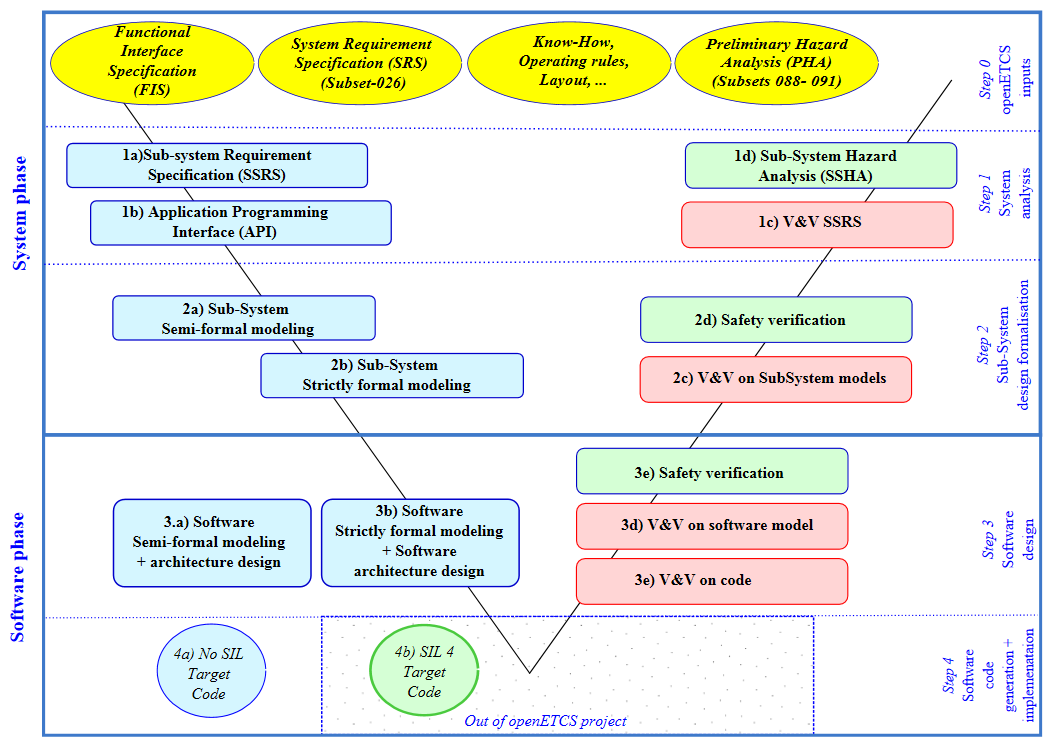
\includegraphics[width=.9\textwidth]{images/ProcessOpenETCS-BeM.png}
  \caption{openETCS Process (rough view)}
  \label{fig:openETCSProcess}
\end{figure}

According figure \ref{fig:openETCSProcess}, for which activities is the mean or tool suitable (see also \citep{D4.1} section 5.1.2 for more details)\footnote{DAS2V : Design Artifact Subject to Verification and Validation, see \citep{D4.1}} ?


\begin{tabular}{|l | c | c | c | c|}
\hline
& \textcolor{green}{Author} & \textcolor{blue}{Assessor 1} & \textcolor{magenta}{Assessor 2} & Total \\
\hline 
1c SSRS Verification & & & &  \\
\hline
1c SSRS Validation & & & &  \\
\hline
2c SFM Verification & & & &  \\
\hline
2c SFM Validation & & & &  \\
\hline
3d SW-SFM Verification & & & &  \\
\hline
3d SW-SFM Validation & & & &  \\
\hline
3d SW-FFM Verification & & & &  \\
\hline
3d SW-FFM Validation & & & &  \\
\hline
3e Code Verification & & & &  \\
\hline
3e Code Validation & & & &  \\
\hline
DAS2V Verification & & & &  \\
\hline
DAS2V Validation & & & &  \\
\hline
Automatic model transformation verification & & & &  \\
\hline
Automatic code generation verification & & & &  \\
\hline
\end{tabular}


\section{Properties}

Which kind of properties or elements are verified or validated by the mean or tool (see also \citep{D4.1} section 4)  ?



\begin{tabular}{|l | c | c | c | c|}
\hline
& \textcolor{green}{Author} & \textcolor{blue}{Assessor 1} & \textcolor{magenta}{Assessor 2} & Total \\
\hline 
Functionalities of the system and sub-system & & & &  \\
\hline
System and sub-system architecture & & & &  \\
\hline
External and internal interfaces of sub-system & & & &  \\
\hline
Software components & & & &  \\
\hline
Performance constraints & & & &  \\
\hline
Safety objectives & & & &  \\
\hline
Functional properties & & & &  \\
\hline
Safety properties & & & &  \\
\hline
\end{tabular}



\section{Verification methods and tools}

Which kind of methods is proposed (see also \citep{D4.1} section 5.3) ?



\begin{tabular}{|l | c | c | c | c|}
\hline
& \textcolor{green}{Author} & \textcolor{blue}{Assessor 1} & \textcolor{magenta}{Assessor 2} & Total \\
\hline 
Reviews & & & &  \\
\hline
Inspections & & & &  \\
\hline
Software Architecture Analysis Method & & & &  \\
\hline
Architecture Tradeoff Analysis Method & & & &  \\
\hline
Model-Based System Integration Testing & & & &  \\
\hline
Model-Based Testing of Generated High-Level Code & & & &  \\
\hline
Abstract Interpretation & & & &  \\
\hline
Deductive Verification & & & &  \\
\hline
Model Checking & & & &  \\
\hline
Correct by Construction Formal Methods & & & &  \\
\hline
Verification with Formal Methods & & & &  \\
\hline
Simulation-based & & & &  \\
\hline
\end{tabular}

\section{Validation means and tools}

The following list of criteria focuss on means and tools to support validation activities, according WP2  requirements :

\begin{tabular}{|l | c | c | c | c|}
\hline
& \textcolor{green}{Author} & \textcolor{blue}{Assessor 1} & \textcolor{magenta}{Assessor 2} & Total \\
\hline 
Simulation-based & & & &  \\
\hline
Step-by-step simulation (D2.6-01-036) & & & &  \\
\hline
Environment emulation (D2.6-01-037 and D2.6-02-080) & & & &  \\
\hline
Time-based test case (D2.6-02-081) & & & &  \\
\hline
Test cases writing (D2.6-01-038) & & & &  \\
\hline
Test cases execution (D2.6-01-038) & & & &  \\
\hline
Test cases storage (D2.6-01-038) & & & &  \\
\hline
Version management of test cases (D2.6-02-082) & & & &  \\
\hline
Test generation from independant test model (D2.6-02-083) & & & &  \\
\hline
Test sequences writing (D2.6-02-084) & & & &  \\
\hline
Test sequences execution (D2.6-02-084) & & & &  \\
\hline
Test sequences storage (D2.6-02-084) & & & &  \\
\hline
\end{tabular}

\section{VnV artifacts}


Concerning the artifacts used or produced by the mean or tool, please to detail:

\paragraph{Input}
    Which is the list of the input artifacts for the mean or tools ?
    
    
\paragraph{Output}
    Which is the list of the output artifacts for the mean or tools ?
    
\paragraph{Syntax}
    Which are the reference documents which give a description of the artifacts syntax  ?
    
\paragraph{Semantic}
    Which are the reference documents which give a description of the artifacts semantic  ?


\paragraph{Integration}
    How these artifacts can be integrated with the elements of the toolchain (language, mangement,...) ?


\section{Detailled Criterias for VnV}

Please  fill only the section concerning the proposed mean or tool, other section can be skipped (see issue \url{https://github.com/openETCS/toolchain/issues/180} for details and discussions)



\subsection{System Modelling simulation}	

\begin{tabular}{|l | c | c | c | c|}
\hline
& \textcolor{green}{Author} & \textcolor{blue}{Assessor 1} & \textcolor{magenta}{Assessor 2} & Total \\
\hline 
User Scenario Modelling & & & &  \\
\hline
Test Case Modelling & & & &  \\
\hline
Test Sequence Modelling & & & &  \\
\hline
\end{tabular}
	
\subsection{System Model Verification}	


\begin{tabular}{|l | c | c | c | c|}
\hline
& \textcolor{green}{Author} & \textcolor{blue}{Assessor 1} & \textcolor{magenta}{Assessor 2} & Total \\
\hline 
Input/ Output checking & & & &  \\
\hline
System Behavior Simulation (Mathematical) & & & &  \\
\hline
System Behavior Simulation (Animated) & & & &  \\
\hline
\end{tabular}


\subsection{Software Model Verification	}


\begin{tabular}{|l | c | c | c | c|}
\hline
& \textcolor{green}{Author} & \textcolor{blue}{Assessor 1} & \textcolor{magenta}{Assessor 2} & Total \\
\hline 
Static Model Verification & & & &  \\
\hline
Property Proofing & & & &  \\
\hline
Dynamic Testing & & & &  \\
\hline
Automatic Test Generation & & & &  \\
\hline
Input/ Output checking & & & &  \\
\hline
Software Behaviour Simulation (Mathematical) & & & &  \\
\hline
Software Behaviour Simulation (Animated) & & & &  \\
\hline
\end{tabular}


\subsection{Source Code}


\begin{tabular}{|l | c | c | c | c|}
\hline
& \textcolor{green}{Author} & \textcolor{blue}{Assessor 1} & \textcolor{magenta}{Assessor 2} & Total \\
\hline 
Traceability to Model & & & &  \\
\hline
\end{tabular}


\subsection{Code Verification	}


\begin{tabular}{|l | c | c | c | c|}
\hline
& \textcolor{green}{Author} & \textcolor{blue}{Assessor 1} & \textcolor{magenta}{Assessor 2} & Total \\
\hline 
Formal Proof & & & &  \\
\hline
Programming by contract & & & &  \\
\hline
Static Analysis & & & &  \\
\hline
Dynamic Analysis & & & &  \\
\hline
Dynamic Testing & & & &  \\
\hline
Automatic Test Generation & & & &  \\
\hline
Performance Testing & & & &  \\
\hline
Interface Testing & & & &  \\
\hline
\end{tabular}

	
\subsection{Validation System/Software/Code/ Validation	}


\begin{tabular}{|l | c | c | c | c|}
\hline
& \textcolor{green}{Author} & \textcolor{blue}{Assessor 1} & \textcolor{magenta}{Assessor 2} & Total \\
\hline 
Test Coverage & & & &  \\
\hline
Use Case Validation of Model & & & &  \\
\hline
Functional or Black-box Testing & & & &  \\
\hline
User Scenario Testing & & & &  \\
\hline
Traceability & & & &  \\
\hline
Schedulability Analyzer / UseCase Check all & & & &  \\
\hline
Schedulability Analyzer / UseCase Check single mode & & & &  \\
\hline

\end{tabular}



\section{Other comments}



\begin{comment}
This section is available for the author or the assessors to  complete the description and criteria.
\end{comment}




\chapter{UPPAAL}
\label{sec:uppaal}

\section{Instructions}

\begin{description}
\item[\textcolor{green}{Author}] Stefan Rieger (TWT)
\item[\textcolor{blue}{Assessor 1}] First assessor of the approaches \todo{Name - Company}
\item[\textcolor{magenta}{Assessor 2}] Second assessor of the approaches \todo{Name - Company}
\end{description}

In the sequel, main text is under the responsibilities of the author.

\begin{author_comment}
Author can add comments using this format at any place.
\end{author_comment}

\begin{assessor1}
First assessor can add comments using this format at any place.
\end{assessor1}

\begin{assessor2}
Second assessor can add comments using this format at any place.
\end{assessor2}

When a note is required, please follow this list (inspired from Technology Readiness Level, see \url{http://en.wikipedia.org/wiki/Technology\_readiness\_level}) :

\begin{description}
\item[0] not recommended / rejected / no integration possible or valuable / not adapted for this topic / not available for this topic
\item[1] weakly recommended / adapted after major improvements / weakly rejected / concept of integration roughly defined / adapted after major improvements / available after major developments
\item[2] recommended / adapted (with light improvements if necessary)  weakly accepted / integration prototyped or defined in details / adapted after small improvements / available after small developments or tests
\item[3] highly recommended / well adapted / strongly accepted / integration done and tested / well adapted to the purpose / available and suitable for the purpose All the notes can be commented under each table.
\item[*] difficult to evaluate with a note (please add a comment under the table)
\end{description}


All the notes can be commented under each table.

This section defines the criteria for the means and tools dedicated to verification and validation activities, in the WP4 workpackage. 

Criteria of this section are defined according \citep{D4.1}.

\section{Presentation}

This section gives a quick presentation of the approach and the tool.

\begin{description}
\item[Name] UPPAAL
\item[Web site] www.uppaal.org
\item[Licence] Academic free or commercial license
\end{description}

\paragraph{Abstract} Uppaal is an integrated tool environment for modeling, validation and verification of real-time systems modeled as networks of timed automata, extended with data types (bounded integers, arrays, etc.).

\paragraph{Publications} Short list of publications on the approach (5 max)
Please refer to \verb|http://dblp.org/search/#query=uppaal|


\section{Common criteria on secondary means and tools}
\label{common}
This section discusses the common criteria of the means and tools according to the project requirements on tools and the results of T7.1.

\subsection{Project and WP2 requirements}

The objectives of this list of criteria is to check if the proposed means and tools meet the main criteria of the project: open-source approaches, usability, modularity, coverage of the objectives,...

According WP2 requirements, give a note for characteristics of the use of the tool (from 0 to 3) :

\begin{tabular}{|l | c | c | c | c|}
\hline
& \textcolor{green}{Author} & \textcolor{blue}{Assessor 1} & \textcolor{magenta}{Assessor 2} & Total \\
\hline 
Open Source (D2.6-02-074) &0 & & &  \\
\hline 
Portability to operating systems (D2.6-02-075) &3 & & &  \\
\hline
Cooperation of tools (D2.6-02-076) &2 & & &  \\
\hline
Robustness (D2.6-02-078) &2* & & & \\
\hline
Modularity (D2.6-02-078.1) &2 & & & \\
\hline
Documentation management (D2.6-02-078.02) &0** & & & \\
\hline
Distributed software development (D2.6-02-078.03)  &0** & & & \\
\hline
Simultaneous multi-users (D2.6-02-078.04)   &0** & & & \\
\hline
Issue tracking (D2.6-02-078.05) &0** & & & \\
\hline
Differences between models (D2.6-02-078.06) &0** & & & \\
\hline
Version management (D2.6-02-078.07) &0** & & & \\
\hline
Concurrent version development (D2.6-02-078.08) &0** & & & \\
\hline
Model-based version control (D2.6-02-078.09) &0** & & & \\
\hline
Role traceability (D2.6-02-078.10) &0** & & & \\
\hline
Safety version traceability (D2.6-02-078.11) &0** & & & \\
\hline
Model traceability (D2.6-02-079) &0** & & & \\
\hline
Tool chain integration &2 & & & \\
\hline
Scalability &*** & & & \\
\hline
User Friendliness &3& & & \\
\hline
\end{tabular}

\begin{author_comment}
\begin{description}
\item[*] Sub-criteria of robustness in D2.6 do not make sense here, e.g., version management is not a sub-criterion to robustness.
\item[**] Out of scope of this tool. The requirements address an tool chain, so other tools should be used to cover these aspects.
\item[***] Scalability is difficult to judge and has not been evaluated. As with most tools for model checking it is important how a system model is specified (e.g., bounded datatypes, etc.).
\end{description}
\end{author_comment}


\subsection{Qualification}

This section discusses how the tool can be classified according EN50128 requirements (D2.6-02-085). Some qualification shall be mandatory  if the tool is involved to design a SIL4 software.


\begin{tabular}{|l | c | c | c | c|}
\hline
& \textcolor{green}{Author} & \textcolor{blue}{Assessor 1} & \textcolor{magenta}{Assessor 2} & Total \\
\hline 
Tool manual (D.2.6-01-42.02) &2* & & &  \\
\hline
Proof of correctness (D.2.6-01-42.03)   &0 & & & \\
\hline
Existing industrial  usage  &** & & & \\
\hline
Model verification &3 & & & \\
\hline
Test generation &2 & & & \\
\hline
Simulation, execution, debugging &2 & & & \\
\hline
Formal proof &3 & & & \\
\hline
\end{tabular}

\begin{author_comment}
The above table is not entirely clear to me. I filled the items 4-7 according to applicability of the tool.
\begin{description}
\item[*] Several tutorial papers available.
\item[**] Not checked in this context.
\end{description}
\end{author_comment}


Which level of tool qualification has been reached or will be reached within the next year ?

\begin{author_comment}
The possible answers below are not aligned with the above question and thus make no sense. The tool is not / will not be pre-qualified by the tool author. Tool qualification by a third party is not possible because the tool is closed source at the moment.
\end{author_comment}

Score :
\begin{description}
\item[3] already qualified for this level
\item[2] qualification possible to this level, but some elements shall be provided
\item[0] qualification not recommended for this level
\end{description}


\begin{tabular}{|l | c | c | c | c|}
\hline
& \textcolor{green}{Author} & \textcolor{blue}{Assessor 1} & \textcolor{magenta}{Assessor 2} & Total \\
\hline 
class T1 & & & &  \\
\hline
class T2   & & & & \\
\hline
class T3  & & & & \\
\hline
\end{tabular}

\paragraph{Other elements for tool certification}


\subsection{Complementarity with primary toolchain}

The objectives of this list of criteria is to check if the proposed means and tools can be easily integrated to the primary toolchain.

\subsubsection{Language}


According to the decisions and the propositions of T7.1, how the mean and approach can be adapted to or can complete the chosen language and methods:

\begin{tabular}{|l | c | c | c | c|}
\hline
& \textcolor{green}{Author} & \textcolor{blue}{Assessor 1} & \textcolor{magenta}{Assessor 2} & Total \\
\hline 
SysML  &2*& & & \\
\hline
Scade method &** & & & \\
\hline
EFS language &** & & & \\
\hline
B Method &** & & & \\
\hline
C language &0 & & & \\
\hline
\end{tabular}

\begin{author_comment}
\begin{description}
\item[*] Due to XML input and output formats it can be adapted to be combined with SysML, e.g., generating timed automata from SysML Statecharts (Acceleo seems suitable for that)
\item[**] I am lacking the information to judge these items regarding direct integration. Please also read my answers below.
\end{description}
\end{author_comment}

\paragraph{SysML}
How the means or tools can complete SysML ?

\begin{author_comment}
\begin{itemize}
  \item Transformation from SysML, e.g., by using Acceleo
  \item Use UPPAAL to simulate and verify timed aspects of the primary model
  \item Timed model checking using a (manual) abstraction of the SysML-Model
  \item Test cases from counter examples
\end{itemize}
\end{author_comment}

\paragraph{Scade, EFS, Classical B}
How the means or tools can complete the current proposals for formal modeling language ?

\begin{author_comment}
\begin{itemize}
  \item Use UPPAAL to simulate and verify timed aspects of the primary model
  \item Timed model checking using a (manual) abstraction of the primary Model
  \item Test cases from counter examples
\end{itemize}
\end{author_comment}

\paragraph{C language}
How the means or tools can complete or be adapted to SIL4 software in C language ?

\begin{author_comment}
This is not the goal in proposing this tool.
\end{author_comment}

\subsubsection{Tools and platforms}

According to the decisions and the propositions of T7.1, how the mean and approach can be integrated to or can complete the chosen tools and platforms:

\begin{author_comment}
This section in my opinion is redundant for UPPAAL, see my answers above (the answers for Eclipse and Papyrus are the same as for SysML).
\end{author_comment}

\begin{tabular}{|l | c | c | c | c|}
\hline
& \textcolor{green}{Author} & \textcolor{blue}{Assessor 1} & \textcolor{magenta}{Assessor 2} & Total \\
\hline 
Eclipse & & & &  \\
\hline
Papyrus  & & & & \\
\hline
Scade & & & & \\
\hline
EFS tools & & & & \\
\hline
B tools & & & & \\
\hline
\end{tabular}


\paragraph{Eclipse}
How the means or tools can be integrated to the Eclipse platform ?

\begin{author_comment}
See comments regarding SysML above.
\end{author_comment}

\paragraph{Papyrus}
How the means or tools can complete  Papyrus ?

\begin{author_comment}
See comments regarding SysML above.
\end{author_comment}


\paragraph{Scade, EFS, Classical B}
How the means or tools can complete the current proposals for formal modeling tools ?

\begin{author_comment}
See comments regarding cade, EFS, Classical B above.
\end{author_comment}


\section{VnV Activities}

The VnV activities are described in details in the verification and Validation Plan  \citep{D4.1}.

\begin{figure}[htb]
  \centering
  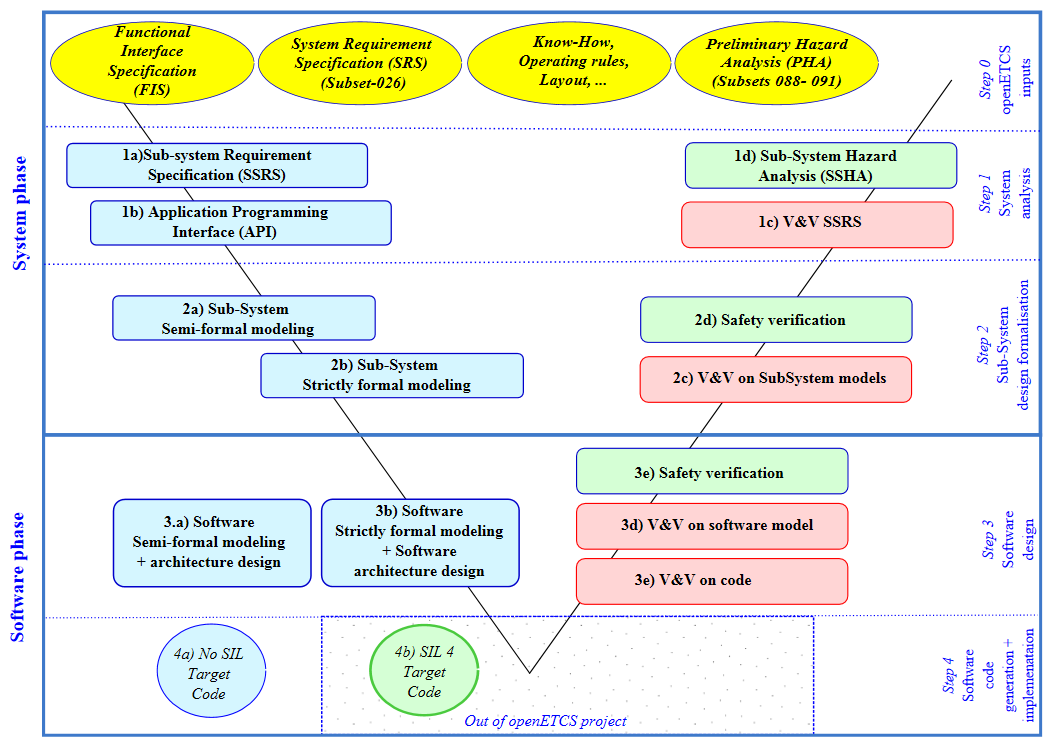
\includegraphics[width=.9\textwidth]{images/ProcessOpenETCS-BeM.png}
  \caption{openETCS Process (rough view)}
  \label{fig:openETCSProcess}
\end{figure}

According figure \ref{fig:openETCSProcess}, for which activities is the mean or tool suitable (see also \citep{D4.1} section 5.1.2 for more details)\footnote{DAS2V : Design Artifact Subject to Verification and Validation, see \citep{D4.1}} ?


\begin{tabular}{|l | c | c | c | c|}
\hline
& \textcolor{green}{Author} & \textcolor{blue}{Assessor 1} & \textcolor{magenta}{Assessor 2} & Total \\
\hline 
1c SSRS Verification & 3& & &  \\
\hline
1c SSRS Validation & 3& & &  \\
\hline
2c SFM Verification & 3& & &  \\
\hline
2c SFM Validation & 3& & &  \\
\hline
3d SW-SFM Verification & 2*& & &  \\
\hline
3d SW-SFM Validation & 2*& & &  \\
\hline
3d SW-FFM Verification & 2*& & &  \\
\hline
3d SW-FFM Validation & 2*& & &  \\
\hline
3e Code Verification & 0& & &  \\
\hline
3e Code Validation & 0& & &  \\
\hline
DAS2V Verification & 3& & &  \\
\hline
DAS2V Validation & 3& & &  \\
\hline
Automatic model transformation verification & 0& & &  \\
\hline
Automatic code generation verification & 0& & &  \\
\hline
\end{tabular}


\begin{author_comment}
\begin{description}
\item[*] Assuming that SW-SFM means Software Semi Formal Model and SW-FFM Software Fully Formal Model
\end{description}
\end{author_comment}

\section{Properties}

Which kind of properties or elements are verified or validated by the mean or tool (see also \citep{D4.1} section 4)  ?



\begin{tabular}{|l | c | c | c | c|}
\hline
& \textcolor{green}{Author} & \textcolor{blue}{Assessor 1} & \textcolor{magenta}{Assessor 2} & Total \\
\hline 
Functionalities of the system and sub-system & 3& & &  \\
\hline
System and sub-system architecture & 0& & &  \\
\hline
External and internal interfaces of sub-system & 0& & &  \\
\hline
Software components & 2& & &  \\
\hline
Performance constraints & 2& & &  \\
\hline
Safety objectives & 3& & &  \\
\hline
Functional properties & 3& & &  \\
\hline
Safety properties & 3& & &  \\
\hline
\end{tabular}



\section{Verification methods and tools}

Which kind of methods are proposed (see also \citep{D4.1} section 5.3) ?



\begin{tabular}{|l | c | c | c | c|}
\hline
& \textcolor{green}{Author} & \textcolor{blue}{Assessor 1} & \textcolor{magenta}{Assessor 2} & Total \\
\hline 
Reviews & 0& & &  \\
\hline
Inspections & 0& & &  \\
\hline
Software Architecture Analysis Method & 0& & &  \\
\hline
Architecture Tradeoff Analysis Method & 0& & &  \\
\hline
Model-Based System Integration Testing & 0& & &  \\
\hline
Model-Based Testing of Generated High-Level Code & 0& & &  \\
\hline
Abstract Interpretation & 0& & &  \\
\hline
Deductive Verification & 0& & &  \\
\hline
Model Checking & 3& & &  \\
\hline
Correct by Construction Formal Methods & 0& & &  \\
\hline
Verification with Formal Methods & 3& & &  \\
\hline
Simulation-based & 2& & &  \\
\hline
\end{tabular}

\section{Validation means and tools}

The following list of criteria focuss on means and tools to support validation activities, according WP2  requirements :

\begin{tabular}{|l | c | c | c | c|}
\hline
& \textcolor{green}{Author} & \textcolor{blue}{Assessor 1} & \textcolor{magenta}{Assessor 2} & Total \\
\hline 
Simulation-based & 3& & &  \\
\hline
Step-by-step simulation (D2.6-01-036) & 3& & &  \\
\hline
Environment emulation (D2.6-01-037 and D2.6-02-080) & 0& & &  \\
\hline
Time-based test case (D2.6-02-081) & 0& & &  \\
\hline
Test cases writing (D2.6-01-038) & 0& & &  \\
\hline
Test cases execution (D2.6-01-038) & 0& & &  \\
\hline
Test cases storage (D2.6-01-038) & 0& & &  \\
\hline
Version management of test cases (D2.6-02-082) & 0& & &  \\
\hline
Test generation from independant test model (D2.6-02-083) & 2& & &  \\
\hline
Test sequences writing (D2.6-02-084) & 0& & &  \\
\hline
Test sequences execution (D2.6-02-084) & 0& & &  \\
\hline
Test sequences storage (D2.6-02-084) & 0& & &  \\
\hline
\end{tabular}

\section{VnV artifacts}


Concerning the artifacts used or produced by the mean or tool, please to detail:

\paragraph{Input}
    Which is the list of the input artifacts for the mean or tools ?

\begin{author_comment}
   Network of timed automata in XML format, this could be a transformed SysML diagram (e.g., statechart).
\end{author_comment}
    
    
\paragraph{Output}
    Which is the list of the output artifacts for the mean or tools ?

\begin{author_comment}
   UPPAAL is an analysis tool that does not provide a single output. Possible results may include:
   \begin{itemize}
     \item Identification of timing issues in the system design or the specification
     \item Specification findings due to simulation/validation of the ETCS specificaiton
     \item Results from model verification with possible error traces / bad states
   \end{itemize}
\end{author_comment}
    
\paragraph{Syntax}
    Which are the reference documents which give a description of the artifacts syntax  ?
    \verb|http://www.it.uu.se/research/group/darts/uppaal/documentation.shtml|
    
\paragraph{Semantic}
    Which are the reference documents which give a description of the artifacts semantic  ?
    \verb|http://www.it.uu.se/research/group/darts/uppaal/documentation.shtml|

\paragraph{Integration}
    How these artifacts can be integrated with the elements of the toolchain (language, mangement,...) ?

\begin{author_comment}
   See above.
\end{author_comment}

\section{Detailled Criterias for VnV}

Please  fill only the section concerning the proposed mean or tool, other section can be skipped (see issue \url{https://github.com/openETCS/toolchain/issues/180} for details and discussions)



\subsection{System Modelling simulation}	

\begin{tabular}{|l | c | c | c | c|}
\hline
& \textcolor{green}{Author} & \textcolor{blue}{Assessor 1} & \textcolor{magenta}{Assessor 2} & Total \\
\hline 
User Scenario Modelling & 2& & &  \\
\hline
Test Case Modelling & 0& & &  \\
\hline
Test Sequence Modelling & 0& & &  \\
\hline
\end{tabular}
	
\subsection{System Model Verification}	


\begin{tabular}{|l | c | c | c | c|}
\hline
& \textcolor{green}{Author} & \textcolor{blue}{Assessor 1} & \textcolor{magenta}{Assessor 2} & Total \\
\hline 
Input/ Output checking &0 & & &  \\
\hline
System Behavior Simulation (Mathematical) & 3& & &  \\
\hline
System Behavior Simulation (Animated) &3 & & &  \\
\hline
\end{tabular}


\subsection{Software Model Verification	}


\begin{tabular}{|l | c | c | c | c|}
\hline
& \textcolor{green}{Author} & \textcolor{blue}{Assessor 1} & \textcolor{magenta}{Assessor 2} & Total \\
\hline 
Static Model Verification & 3& & &  \\
\hline
Property Proofing &3 & & &  \\
\hline
Dynamic Testing &0 & & &  \\
\hline
Automatic Test Generation & 0& & &  \\
\hline
Input/ Output checking & 0& & &  \\
\hline
Software Behaviour Simulation (Mathematical) & 2& & &  \\
\hline
Software Behaviour Simulation (Animated) & 2& & &  \\
\hline
\end{tabular}


\subsection{Source Code}


\begin{tabular}{|l | c | c | c | c|}
\hline
& \textcolor{green}{Author} & \textcolor{blue}{Assessor 1} & \textcolor{magenta}{Assessor 2} & Total \\
\hline 
Traceability to Model & & & &  \\
\hline
\end{tabular}


\subsection{Code Verification	}


\begin{tabular}{|l | c | c | c | c|}
\hline
& \textcolor{green}{Author} & \textcolor{blue}{Assessor 1} & \textcolor{magenta}{Assessor 2} & Total \\
\hline 
Formal Proof & & & &  \\
\hline
Programming by contract & & & &  \\
\hline
Static Analysis & & & &  \\
\hline
Dynamic Analysis & & & &  \\
\hline
Dynamic Testing & & & &  \\
\hline
Automatic Test Generation & & & &  \\
\hline
Performance Testing & & & &  \\
\hline
Interface Testing & & & &  \\
\hline
\end{tabular}

	
\subsection{Validation System/Software/Code/ Validation	}


\begin{tabular}{|l | c | c | c | c|}
\hline
& \textcolor{green}{Author} & \textcolor{blue}{Assessor 1} & \textcolor{magenta}{Assessor 2} & Total \\
\hline 
Test Coverage & & & &  \\
\hline
Use Case Validation of Model & & & &  \\
\hline
Functional or Black-box Testing & & & &  \\
\hline
User Scenario Testing & & & &  \\
\hline
Traceability & & & &  \\
\hline
Schedulability Analyzer / UseCase Check all & & & &  \\
\hline
Schedulability Analyzer / UseCase Check single mode & & & &  \\
\hline

\end{tabular}



\section{Other comments}



\begin{comment}
This section is available for the author or the assessors to  complete the description and criteria.
\end{comment}




\chapter{Rodin}
\label{sec:rodin}

No results of evaluation.
Slides available on github \url{https://github.com/openETCS/model-evaluation/blob/master/Telco_Secondary_slides/Systerel_Event-B.pdf}.


\chapter{Tools for classical B}
\label{sec:classicalB}

No results of evaluation.


Slides available on github \url{https://github.com/openETCS/model-evaluation/blob/master/Telco_Secondary_slides/ClassicalB_VnV.pdf}.


\chapter{CPN Tools}
\label{sec:cpntools}

\section{Instructions}

\begin{description}
\item[\textcolor{green}{Author}] Stefan Rieger (TWT), Jan Welte (TUBS)
\item[\textcolor{blue}{Assessor 1}] First assessor of the approaches \todo{Name - Company}
\item[\textcolor{magenta}{Assessor 2}] Second assessor of the approaches \todo{Name - Company}
\end{description}

In the sequel, main text is under the responsibilities of the author.

\begin{author_comment}
Author can add comments using this format at any place.
\end{author_comment}

\begin{assessor1}
First assessor can add comments using this format at any place.
\end{assessor1}

\begin{assessor2}
Second assessor can add comments using this format at any place.
\end{assessor2}

When a note is required, please follow this list (inspired from Technology Readiness Level, see \url{http://en.wikipedia.org/wiki/Technology\_readiness\_level}) :

\begin{description}
\item[0] not recommended / rejected / no integration possible or valuable / not adapted for this topic / not available for this topic
\item[1] weakly recommended / adapted after major improvements / weakly rejected / concept of integration roughly defined / adapted after major improvements / available after major developments
\item[2] recommended / adapted (with light improvements if necessary)  weakly accepted / integration prototyped or defined in details / adapted after small improvements / available after small developments or tests
\item[3] highly recommended / well adapted / strongly accepted / integration done and tested / well adapted to the purpose / available and suitable for the purpose All the notes can be commented under each table.
\item[*] difficult to evaluate with a note (please add a comment under the table)
\end{description}


All the notes can be commented under each table.

This section defines the criteria for the means and tools dedicated to verification and validation activities, in the WP4 workpackage. 

Criteria of this section are defined according \citep{D4.1}.

\section{Presentation}

This section gives a quick presentation of the approach and the tool.

\begin{description}
\item[Name] CPN Tools
\item[Website] http://cpntools.org/
\item[Licence] Open Source (GPL/LGPL)
\end{description}

\paragraph{Abstract} CPN Tools is a tool for editing, simulating, and analyzing Colored Petri nets.

The tool features incremental syntax checking and code generation, which take place while a net is being constructed. A fast simulator efficiently handles untimed and timed nets. Full and partial state spaces can be generated and analyzed, and a standard state space report contains information, such as boundedness properties and liveness properties.

\paragraph{Publications} Please refer to http://cpntools.org/publications


\section{Common criteria on secondary means and tools}
\label{common}
This section discusses the common criteria of the means and tools according to the project requirements on tools and the results of T7.1.

\subsection{Project and WP2 requirements}

The objectives of this list of criteria is to check if the proposed means and tools meet the main criteria of the project: open-source approaches, usability, modularity, coverage of the objectives,...

According WP2 requirements, give a note for characteristics of the use of the tool (from 0 to 3) :

\begin{tabular}{|l | c | c | c | c|}
\hline
& \textcolor{green}{Author} & \textcolor{blue}{Assessor 1} & \textcolor{magenta}{Assessor 2} & Total \\
\hline 
Open Source (D2.6-02-074) & 3& & &  \\
\hline 
Portability to operating systems (D2.6-02-075) & 2& & &  \\
\hline
Cooperation of tools (D2.6-02-076) & 2& & &  \\
\hline
Robustness (D2.6-02-078) & 2*& & & \\
\hline
Modularity (D2.6-02-078.1) &3 & & & \\
\hline
Documentation management (D2.6-02-078.02) &0** & & & \\
\hline
Distributed software development (D2.6-02-078.03)  &0** & & & \\
\hline
Simultaneous multi-users (D2.6-02-078.04)   &0** & & & \\
\hline
Issue tracking (D2.6-02-078.05) &0** & & & \\
\hline
Differences between models (D2.6-02-078.06) &0** & & & \\
\hline
Version management (D2.6-02-078.07) &0** & & & \\
\hline
Concurrent version development (D2.6-02-078.08) &0** & & & \\
\hline
Model-based version control (D2.6-02-078.09) &0** & & & \\
\hline
Role traceability (D2.6-02-078.10) &0** & & & \\
\hline
Safety version traceability (D2.6-02-078.11) &0** & & & \\
\hline
Model traceability (D2.6-02-079) &0** & & & \\
\hline
Tool chain integration &2** & & & \\
\hline
Scalability &2*** & & & \\
\hline
User Friendliness &3 & & & \\
\hline
\end{tabular}

\begin{author_comment}
\begin{description}
\item[*] Sub-criteria of robustness in D2.6 do not make sense here, e.g., a tool is not robust if it supports version management.
\item[**] Out of scope of this tool. The requirements address an tool chain, so other tools should be used to cover these aspects.
\item[***] For simulation it seems to scale well. State space generation/exhaustive verification scalability was not evaluated so far.
\end{description}
\end{author_comment}


\subsection{Qualification}

This section discusses how the tool can be classified according EN50128 requirements (D2.6-02-085). Some qualification shall be mandatory  if the tool is involved to design a SIL4 software.


\begin{tabular}{|l | c | c | c | c|}
\hline
& \textcolor{green}{Author} & \textcolor{blue}{Assessor 1} & \textcolor{magenta}{Assessor 2} & Total \\
\hline 
Tool manual (D.2.6-01-42.02) &3& & &  \\
\hline
Proof of correctness (D.2.6-01-42.03)   &0& & & \\
\hline
Existing industrial  usage  &*& & & \\
\hline
Model verification &3 & & & \\
\hline
Test generation &2& & & \\
\hline
Simulation, execution, debugging &3& & & \\
\hline
Formal proof &3& & & \\
\hline
\end{tabular}

\begin{author_comment}
The above table is not entirely clear to me. I filled the items 4-7 according to applicability of the tool.
\end{author_comment}

Which level of tool qualification has been reached or will be reached within the next year ?

\begin{author_comment}
The possible answers below are not aligned with the above question and thus make no sense. This is an open source tool that is not / will not be pre-qualified by the tool author (as is, e.g., gcc).
\end{author_comment}


Score :
\begin{description}
\item[3] already qualified for this level
\item[2] qualification possible to this level, but some elements shall be provided
\item[0] qualification not recommended for this level
\end{description}


\begin{tabular}{|l | c | c | c | c|}
\hline
& \textcolor{green}{Author} & \textcolor{blue}{Assessor 1} & \textcolor{magenta}{Assessor 2} & Total \\
\hline 
class T1 & & & &  \\
\hline
class T2   & & & & \\
\hline
class T3  & & & & \\
\hline
\end{tabular}



\paragraph{Other elements for tool certification}


\subsection{Complementarity with primary toolchain}

The objectives of this list of criteria is to check if the proposed means and tools can be easily integrated to the primary toolchain.

\subsubsection{Language}


According to the decisions and the propositions of T7.1, how the mean and approach can be adapted to or can complete the chosen language and methods:

\begin{tabular}{|l | c | c | c | c|}
\hline
& \textcolor{green}{Author} & \textcolor{blue}{Assessor 1} & \textcolor{magenta}{Assessor 2} & Total \\
\hline 
SysML  &2*& & & \\
\hline
Scade method &** & & & \\
\hline
EFS language &** & & & \\
\hline
B Method &** & & & \\
\hline
C language &1* & & & \\
\hline
\end{tabular}

\begin{author_comment}
\begin{description}
\item[*] Due to XML input and output formats it can be adapted to be combined with SysML, e.g., generating CPNs from SysML Statecharts (Acceleo seems suitable for that) or C-Code from CPN models (we do not plan this for the project; it is not necessary in the context of the project).
\item[**] I am lacking the information to judge these items regarding direct integration. Please also read my answers below.
\end{description}
\end{author_comment}

\paragraph{SysML}
How the means or tools can complete SysML ?

\begin{author_comment}
\begin{itemize}
  \item Transformation from SysML, e.g., by using Acceleo
  \item Use CPN model to simulate and debug SysML models
  \item Model checking using an abstraction of the SysML-Model (behavioural parts)
  \item Independent test model to validate primary SysML model
  \item Visualisation of system behaviour
\end{itemize}
\end{author_comment}


\paragraph{Scade, EFS, Classical B}
How the means or tools can complete the current proposals for formal modeling language ?

\begin{author_comment}
\begin{itemize}
  \item Model checking using an abstraction of the primary models (behavioural parts)
  \item Independent test model to validate primary model
  \item Visualisation of system behaviour
\end{itemize}
\end{author_comment}

\paragraph{C language}
How the means or tools can complete or be adapted to SIL4 software in C language ?

\begin{author_comment}
This is not the goal in proposing this tool.
\end{author_comment}

\subsubsection{Tools and platforms}

According to the decisions and the propositions of T7.1, how the mean and approach can be integrated to or can complete the chosen tools and platforms:

\begin{author_comment}
This section in my opinion is redundant for CPN Tools, see my answers above (the answers for Eclipse and Papyrus are the same as for SysML).
\end{author_comment}

\begin{tabular}{|l | c | c | c | c|}
\hline
& \textcolor{green}{Author} & \textcolor{blue}{Assessor 1} & \textcolor{magenta}{Assessor 2} & Total \\
\hline 
Eclipse & & & &  \\
\hline
Papyrus  & & & & \\
\hline
Scade & & & & \\
\hline
EFS tools & & & & \\
\hline
B tools & & & & \\
\hline
\end{tabular}

\paragraph{Eclipse}
How the means or tools can be integrated to the Eclipse platform ?

\begin{author_comment}
See comments regarding SysML above.
\end{author_comment}

\paragraph{Papyrus}
How the means or tools can complete  Papyrus ?

\begin{author_comment}
See comments regarding SysML above.
\end{author_comment}


\paragraph{Scade, EFS, Classical B}
How the means or tools can complete the current proposals for formal modeling tools ?

\begin{author_comment}
See comments regarding cade, EFS, Classical B above.
\end{author_comment}


\section{VnV Activities}

The VnV activities are described in details in the verification and Validation Plan  \citep{D4.1}.

\begin{figure}[htb]
  \centering
  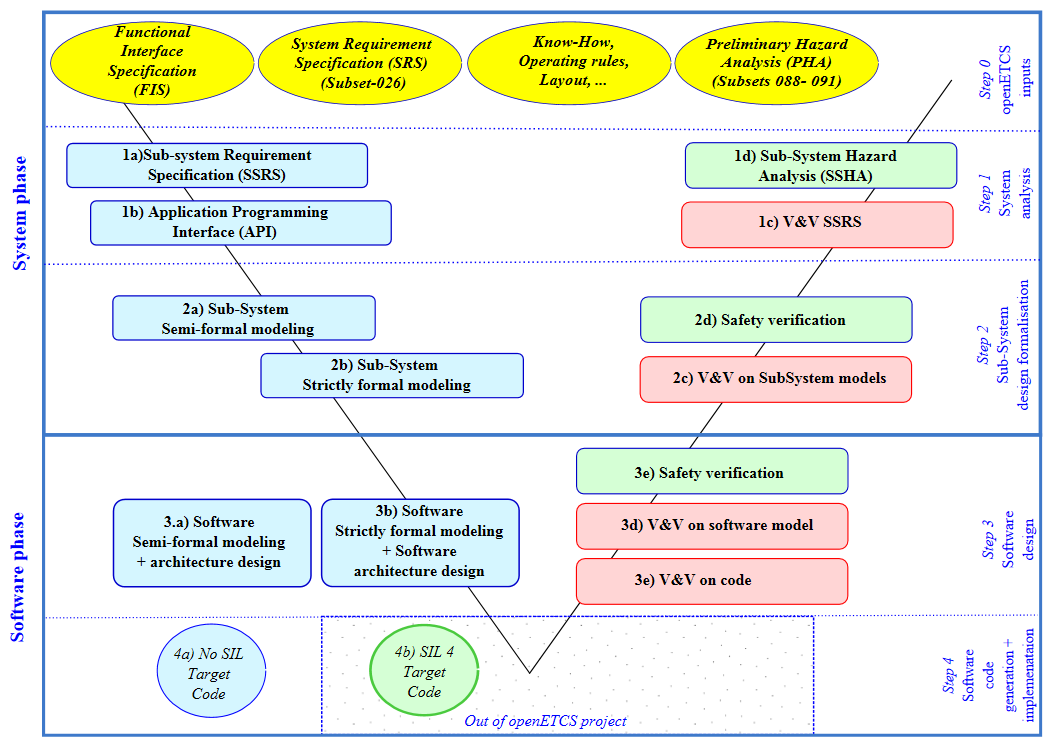
\includegraphics[width=.9\textwidth]{images/ProcessOpenETCS-BeM.png}
  \caption{openETCS Process (rough view)}
  \label{fig:openETCSProcess}
\end{figure}

According figure \ref{fig:openETCSProcess}, for which activities is the mean or tool suitable (see also \citep{D4.1} section 5.1.2 for more details)\footnote{DAS2V : Design Artifact Subject to Verification and Validation, see \citep{D4.1}} ?


\begin{tabular}{|l | c | c | c | c|}
\hline
& \textcolor{green}{Author} & \textcolor{blue}{Assessor 1} & \textcolor{magenta}{Assessor 2} & Total \\
\hline 
1c SSRS Verification & 3& & &  \\
\hline
1c SSRS Validation & 3& & &  \\
\hline
2c SFM Verification & 3& & &  \\
\hline
2c SFM Validation & 3& & &  \\
\hline
3d SW-SFM Verification &3 & & &  \\
\hline
3d SW-SFM Validation & 3& & &  \\
\hline
3d SW-FFM Verification & 3& & &  \\
\hline
3d SW-FFM Validation & 3& & &  \\
\hline
3e Code Verification &0 & & &  \\
\hline
3e Code Validation &0 & & &  \\
\hline
DAS2V Verification &3 & & &  \\
\hline
DAS2V Validation &3 & & &  \\
\hline
Automatic model transformation verification &0 & & &  \\
\hline
Automatic code generation verification &0 & & &  \\
\hline
\end{tabular}


\section{Properties}

Which kind of properties or elements are verified or validated by the mean or tool (see also \citep{D4.1} section 4)  ?



\begin{tabular}{|l | c | c | c | c|}
\hline
& \textcolor{green}{Author} & \textcolor{blue}{Assessor 1} & \textcolor{magenta}{Assessor 2} & Total \\
\hline 
Functionalities of the system and sub-system & 3& & &  \\
\hline
System and sub-system architecture & 0& & &  \\
\hline
External and internal interfaces of sub-system & 0& & &  \\
\hline
Software components & 3& & &  \\
\hline
Performance constraints & 2*& & &  \\
\hline
Safety objectives & 3& & &  \\
\hline
Functional properties & 3& & &  \\
\hline
Safety properties & 3& & &  \\
\hline
\end{tabular}

\begin{author_comment}
 * By introducing timing
\end{author_comment}


\section{Verification methods and tools}

Which kind of methods is proposed (see also \citep{D4.1} section 5.3) ?



\begin{tabular}{|l | c | c | c | c|}
\hline
& \textcolor{green}{Author} & \textcolor{blue}{Assessor 1} & \textcolor{magenta}{Assessor 2} & Total \\
\hline 
Reviews & 0& & &  \\
\hline
Inspections & 0& & &  \\
\hline
Software Architecture Analysis Method & 0& & &  \\
\hline
Architecture Tradeoff Analysis Method & 0& & &  \\
\hline
Model-Based System Integration Testing & 0& & &  \\
\hline
Model-Based Testing of Generated High-Level Code & 0& & &  \\
\hline
Abstract Interpretation & 0& & &  \\
\hline
Deductive Verification & 0& & &  \\
\hline
Model Checking & 3& & &  \\
\hline
Correct by Construction Formal Methods & 0& & &  \\
\hline
Verification with Formal Methods & 3& & &  \\
\hline
Simulation-based & 3& & &  \\
\hline
\end{tabular}

\section{Validation means and tools}

The following list of criteria focus on means and tools to support validation activities, according to WP2  requirements :

\begin{tabular}{|l | c | c | c | c|}
\hline
& \textcolor{green}{Author} & \textcolor{blue}{Assessor 1} & \textcolor{magenta}{Assessor 2} & Total \\
\hline 
Simulation-based & 3& & &  \\
\hline
Step-by-step simulation (D2.6-01-036) & 3& & &  \\
\hline
Environment emulation (D2.6-01-037 and D2.6-02-080) & 0& & &  \\
\hline
Time-based test case (D2.6-02-081) & 2& & &  \\
\hline
Test cases writing (D2.6-01-038) & 0& & &  \\
\hline
Test cases execution (D2.6-01-038) & 0& & &  \\
\hline
Test cases storage (D2.6-01-038) & 0& & &  \\
\hline
Version management of test cases (D2.6-02-082) & 0& & &  \\
\hline
Test generation from independant test model (D2.6-02-083) & 2& & &  \\
\hline
Test sequences writing (D2.6-02-084) & 0& & &  \\
\hline
Test sequences execution (D2.6-02-084) & 0& & &  \\
\hline
Test sequences storage (D2.6-02-084) & 0& & &  \\
\hline
\end{tabular}

\section{VnV artifacts}


Concerning the artifacts used or produced by the mean or tool, please to detail:

\paragraph{Input}
    Which is the list of the input artifacts for the mean or tools ?

\begin{author_comment}
   CPN in XML format, this could be a transformed SysML diagram (e.g., statechart). CPN Tools is based on the functional language ML and thus the input may contain ML elements.
\end{author_comment}
    
    
\paragraph{Output}
    Which is the list of the output artifacts for the mean or tools ?

\begin{author_comment}
   CPN Tools is an analysis tool that does not provide a single output. Possible results of a CPN-analysis may include:
   \begin{itemize}
     \item Specification findings due to simulation/validation of the ETCS specificaiton
     \item Results from model verification with possible error traces / bad states
     \item Visualisation of system execution
   \end{itemize}
\end{author_comment}


    
\paragraph{Syntax}
    Which are the reference documents which give a description of the artifacts syntax  ?

\begin{author_comment}
   See http://cpntools.org/documentation/start
\end{author_comment}
    
\paragraph{Semantic}
    Which are the reference documents which give a description of the artifacts semantic  ?

\begin{author_comment}
   See http://cpntools.org/documentation/start
\end{author_comment}

\paragraph{Integration}
    How these artifacts can be integrated with the elements of the toolchain (language, mangement,...) ?

\begin{author_comment}
   See above.
\end{author_comment}


\section{Detailled Criteria for VnV}

Please  fill only the section concerning the proposed mean or tool, other section can be skipped (see issue \url{https://github.com/openETCS/toolchain/issues/180} for details and discussions)



\subsection{System Modelling simulation}	

\begin{tabular}{|l | c | c | c | c|}
\hline
& \textcolor{green}{Author} & \textcolor{blue}{Assessor 1} & \textcolor{magenta}{Assessor 2} & Total \\
\hline 
User Scenario Modelling & 3& & &  \\
\hline
Test Case Modelling & 3& & &  \\
\hline
Test Sequence Modelling & 0& & &  \\
\hline
\end{tabular}
	
\subsection{System Model Verification}	


\begin{tabular}{|l | c | c | c | c|}
\hline
& \textcolor{green}{Author} & \textcolor{blue}{Assessor 1} & \textcolor{magenta}{Assessor 2} & Total \\
\hline 
Input/ Output checking & 3& & &  \\
\hline
System Behavior Simulation (Mathematical) & 3& & &  \\
\hline
System Behavior Simulation (Animated) & 3& & &  \\
\hline
\end{tabular}


\subsection{Software Model Verification	}


\begin{tabular}{|l | c | c | c | c|}
\hline
& \textcolor{green}{Author} & \textcolor{blue}{Assessor 1} & \textcolor{magenta}{Assessor 2} & Total \\
\hline 
Static Model Verification & 3& & &  \\
\hline
Property Proofing & 3& & &  \\
\hline
Dynamic Testing & 0& & &  \\
\hline
Automatic Test Generation & 0& & &  \\
\hline
Input/ Output checking & 0& & &  \\
\hline
Software Behaviour Simulation (Mathematical) & 3& & &  \\
\hline
Software Behaviour Simulation (Animated) & 3& & &  \\
\hline
\end{tabular}


\subsection{Source Code}


\begin{tabular}{|l | c | c | c | c|}
\hline
& \textcolor{green}{Author} & \textcolor{blue}{Assessor 1} & \textcolor{magenta}{Assessor 2} & Total \\
\hline 
Traceability to Model & & & &  \\
\hline
\end{tabular}


\subsection{Code Verification	}


\begin{tabular}{|l | c | c | c | c|}
\hline
& \textcolor{green}{Author} & \textcolor{blue}{Assessor 1} & \textcolor{magenta}{Assessor 2} & Total \\
\hline 
Formal Proof & & & &  \\
\hline
Programming by contract & & & &  \\
\hline
Static Analysis & & & &  \\
\hline
Dynamic Analysis & & & &  \\
\hline
Dynamic Testing & & & &  \\
\hline
Automatic Test Generation & & & &  \\
\hline
Performance Testing & & & &  \\
\hline
Interface Testing & & & &  \\
\hline
\end{tabular}

	
\subsection{Validation System/Software/Code/ Validation	}


\begin{tabular}{|l | c | c | c | c|}
\hline
& \textcolor{green}{Author} & \textcolor{blue}{Assessor 1} & \textcolor{magenta}{Assessor 2} & Total \\
\hline 
Test Coverage & & & &  \\
\hline
Use Case Validation of Model & 3& & &  \\
\hline
Functional or Black-box Testing & & & &  \\
\hline
User Scenario Testing & & & &  \\
\hline
Traceability & & & &  \\
\hline
Schedulability Analyzer / UseCase Check all & & & &  \\
\hline
Schedulability Analyzer / UseCase Check single mode & & & &  \\
\hline

\end{tabular}



\section{Other comments}



\begin{comment}
This section is available for the author or the assessors to  complete the description and criteria.
\end{comment}




\chapter{Matelo}
\label{sec:matelo}

\section{Instructions}

\begin{description}
\item[\textcolor{green}{Author}] Author of the approaches description  \todo{Name -  Company}
\item[\textcolor{blue}{Assessor 1}] First assessor of the approaches \todo{Name - Company}
\item[\textcolor{magenta}{Assessor 2}] Second assessor of the approaches \todo{Name - Company}
\end{description}

In the sequel, main text is under the responsibilities of the author.

\begin{author_comment}
Author can add comments using this format at any place.
\end{author_comment}

\begin{assessor1}
First assessor can add comments using this format at any place.
\end{assessor1}

\begin{assessor2}
Second assessor can add comments using this format at any place.
\end{assessor2}

When a note is required, please follow this list :
\begin{description}
\item[0] not recommended, not adapted, rejected
\item[1] weakly recommended, adapted after major improvements, weakly rejected
\item[2] recommended, adapted (with light improvements if necessary)  weakly accepted
\item[3] highly recommended, well adapted,strongly accepted
\item[*] difficult to evaluate with a note (please add a comment under the table)
\end{description}

All the notes can be commented under each table.

\section{Presentation}

This section gives a quick presentation of the approach and the tool.

\begin{description}
\item[Name] \todo{Name of the approach and the tool}
\item[Web site] \todo{if available, how to  find information}
\item[Licence] \todo{Kind of licence}
\end{description}

\paragraph{Abstract} Short abstract on the approach and tool (10 lines max)

\paragraph{Publications} Short list of publications on the approach (5 max)


For which activities are dedicaded the means or tools (give a note from 0 to  3) :

\begin{tabular}{|l | c | c | c | c|}
\hline
& \textcolor{green}{Author} & \textcolor{blue}{Assessor 1} & \textcolor{magenta}{Assessor 2} & Total \\
\hline 
Data Management & & & &  \\
\hline
Function Management & & & & \\
\hline
Requirement Management & & & & \\
\hline
Version Management & & & & \\
\hline
Other (give details below) & & & & \\
\hline
\end{tabular}

According the results of this table, some of the following sections can be skipped.

\section{Common criteria on secondary means and tools}
\label{common}
This section discusses the common criteria of the means and tools according to the project requirements on tools and the results of T7.1.

\subsection{Project and WP2 requirements}

The objectives of this list of criteria is to check if the proposed means and tools meet the main criteria of the project: open-source approaches, usability, modularity, coverage of the objectives,...

According WP2 requirements, give a note for characteristics of the use of the tool (from 0 to 3) :

\begin{tabular}{|l | c | c | c | c|}
\hline
& \textcolor{green}{Author} & \textcolor{blue}{Assessor 1} & \textcolor{magenta}{Assessor 2} & Total \\
\hline 
Open Source (D2.6-02-074) & & & &  \\
\hline 
Portability to operating systems (D2.6-02-075) & & & &  \\
\hline
Cooperation of tools (D2.6-02-076) & & & &  \\
\hline
Robustness (D2.6-02-078) & & & & \\
\hline
Modularity (D2.6-02-078.1) & & & & \\
\hline
Documentation management (D2.6-02-078.02) & & & & \\
\hline
Distributed software development (D2.6-02-078.03)  & & & & \\
\hline
Simultaneous multi-users (D2.6-02-078.04)   & & & & \\
\hline
Issue tracking (D2.6-02-078.05) & & & & \\
\hline
Differences between models (D2.6-02-078.06) & & & & \\
\hline
Version management (D2.6-02-078.07) & & & & \\
\hline
Concurrent version development (D2.6-02-078.08) & & & & \\
\hline
Model-based version control (D2.6-02-078.09) & & & & \\
\hline
Role traceability (D2.6-02-078.10) & & & & \\
\hline
Safety version traceability (D2.6-02-078.11) & & & & \\
\hline
Model traceability (D2.6-02-079) & & & & \\
\hline
Tool chain integration & & & & \\
\hline
Scalability & & & & \\
\hline
User Friendliness & & & & \\
\hline
\end{tabular}



\subsection{Qualification}

This section discusses how the tool can be classified according EN50128 requirements (D2.6-02-085). Some qualification shall be mandatory  if the tool is involved to design a SIL4 software.


\begin{tabular}{|l | c | c | c | c|}
\hline
& \textcolor{green}{Author} & \textcolor{blue}{Assessor 1} & \textcolor{magenta}{Assessor 2} & Total \\
\hline 
Tool manual (D.2.6-01-42.02) & & & &  \\
\hline
Proof of correctness (D.2.6-01-42.03)   & & & & \\
\hline
Existing industrial  usage  & & & & \\
\hline
Model verification & & & & \\
\hline
Test generation & & & & \\
\hline
Simulation, execution, debugging & & & & \\
\hline
Formal proof & & & & \\
\hline
\end{tabular}


Which level of tool qualification has been reached or will be reached within the next year ?

Score :
\begin{description}
\item[3] already qualified for this level
\item[2] qualification possible to this level, but some elements shall be provided
\item[0] qualification not recommended for this level
\end{description}


\begin{tabular}{|l | c | c | c | c|}
\hline
& \textcolor{green}{Author} & \textcolor{blue}{Assessor 1} & \textcolor{magenta}{Assessor 2} & Total \\
\hline 
class T1 & & & &  \\
\hline
class T2   & & & & \\
\hline
class T3  & & & & \\
\hline
\end{tabular}

\paragraph{Other elements for tool certification}


\section{Complementarity with primary toolchain}

The objectives of this list of criteria is to check if the proposed means and tools can be easily integrated to the primary toolchain.

\subsection{Language}


According to the decisions and the propositions of T7.1, how the mean and approach can be adapted to or can complete the chosen language and methods:

\begin{tabular}{|l | c | c | c | c|}
\hline
& \textcolor{green}{Author} & \textcolor{blue}{Assessor 1} & \textcolor{magenta}{Assessor 2} & Total \\
\hline 
SysML  & & & & \\
\hline
Scade method & & & & \\
\hline
EFS language & & & & \\
\hline
B Method & & & & \\
\hline
C language & & & & \\
\hline
\end{tabular}

\paragraph{SysML}
How the means or tools can complete SysML ?


\paragraph{Scade, EFS, Classical B}
How the means or tools can complete the current proposals for formal modeling language ?

\paragraph{C language}
How the means or tools can complete or be adapted to SIL4 software in C language ?

\subsection{Tools and platforms}

According to the decisions and the propositions of T7.1, how the mean and approach can be integrated to or can complete the chosen tools and platforms:

\begin{tabular}{|l | c | c | c | c|}
\hline
& \textcolor{green}{Author} & \textcolor{blue}{Assessor 1} & \textcolor{magenta}{Assessor 2} & Total \\
\hline 
Eclipse & & & &  \\
\hline
Papyrus  & & & & \\
\hline
Scade & & & & \\
\hline
EFS tools & & & & \\
\hline
B tools & & & & \\
\hline
\end{tabular}


\paragraph{Eclipse}
How the means or tools can be integrated to the Eclipse platform ?

\paragraph{Papyrus}
How the means or tools can complete  Papyrus ?


\paragraph{Scade, EFS, Classical B}
How the means or tools can complete the current proposals for formal modeling tools ?


\section{Means and tools for data, function and requirement management}
\label{sec:management}


This section defines the criteria for the means and tools dedicated to data, function and requirement management. These activities are shared by the work packages WP3, WP4 and the activities dedicated to  SSRS.
These means and tools shall integrate the primary toolchain to  complete its gap and facilitate the integration of different activities. First of all, they  allow the management of a common repository of data, functions and requirements, shared between the models (from SSRS informal specification to code) and the verification and validation activities.  
Then, they shall support traceability of requirements between models and activities, and facilitate the verification of the traceability.
Besides they shall support the design of SIL4 software with model comparison or document production facilities, and version management.

\subsection{Management activities}

Which activites, linked to help the management of SSRS definition and whole process are covered by the mean or tool  ?

\begin{tabular}{|l | c | c | c | c|}
\hline
& \textcolor{green}{Author} & \textcolor{blue}{Assessor 1} & \textcolor{magenta}{Assessor 2} & Total \\
\hline 
Requirement capturing & & & &  \\
\hline
Requirement management  & & & & \\
\hline
Data management & & & & \\
\hline
Function management & & & & \\
\hline
Requirement traceability  & & & & \\
\hline
Model traceability & & & & \\
\hline
Function architecture & & & & \\
\hline
Version management & & & & \\
\hline
Model comparison & & & & \\
\hline
Documentation production & & & & \\
\hline
Others (give details) & & & & \\
\hline
\end{tabular}


\subsection{Input Artifacts}

Which artifacts are used as input of the mean or tool  ? 


\begin{tabular}{|l | c | c | c | c|}
\hline
& \textcolor{green}{Author} & \textcolor{blue}{Assessor 1} & \textcolor{magenta}{Assessor 2} & Total \\
\hline 
Informal description & & & &  \\
\hline
Structured description & & & & \\
\hline
Spread sheet & & & & \\
\hline
XML files & & & & \\
\hline
EFS model & & & & \\
\hline
DSL & & & & \\
\hline
Others (give details) & & & & \\
\hline
\end{tabular}



\subsection{Output Artifacts}

Which artifacts are used as output of the mean or tool  ? 


\begin{tabular}{|l | c | c | c | c|}
\hline
& \textcolor{green}{Author} & \textcolor{blue}{Assessor 1} & \textcolor{magenta}{Assessor 2} & Total \\
\hline 
Informal description & & & &  \\
\hline
Structured description & & & & \\
\hline
Spread sheet & & & & \\
\hline
XML files & & & & \\
\hline
EFS model & & & & \\
\hline
DSL & & & & \\
\hline
Others (give details) & & & & \\
\hline
\end{tabular}


\subsection{Requirement Management}

This section is link to reauirement definition and management activities.

Are these criteria coverd by the tool or mean ? 


\begin{tabular}{|l | c | c | c | c|}
\hline
& \textcolor{green}{Author} & \textcolor{blue}{Assessor 1} & \textcolor{magenta}{Assessor 2} & Total \\
\hline 
Editing of Textual Requirements & & & &  \\
\hline
Represent Relations between Req (Textual-Based) & & & & \\
\hline
Represent Relations between Req (Modelling-Based) & & & & \\
\hline
Glossary and Abbreviation handling (Linked to Req)) & & & & \\
\hline
Traceability of Textual Requirements to Modelling & & & & \\
\hline
Import/Export of Industrial Standard Data (e.g., REQIF) & & & & \\
\hline
Documentation generation & & & &  \\
\hline
Search and Filtering functions & & & & \\
\hline
Others (give details) & & & & \\
\hline
\end{tabular}



\section{Other comments}



\begin{comment}
This section is available for the author or the assessors to  complete the description and criteria.
\end{comment}




\chapter{RT-Tester}
\label{sec:rttester}

No results of evaluation.



\chapter{Fiacre and Tina}
\label{sec:fiacre}


No results of evaluation.

\chapter{Frama-C}
\label{sec:framaC}

\section{Instructions}

\begin{description}
\item[\textcolor{green}{Author}] Author of the approaches description  \todo{Name -  Company}
\item[\textcolor{blue}{Assessor 1}] First assessor of the approaches \todo{Name - Company}
\item[\textcolor{magenta}{Assessor 2}] Second assessor of the approaches \todo{Name - Company}
\end{description}

In the sequel, main text is under the responsibilities of the author.

\begin{author_comment}
Author can add comments using this format at any place.
\end{author_comment}

\begin{assessor1}
First assessor can add comments using this format at any place.
\end{assessor1}

\begin{assessor2}
Second assessor can add comments using this format at any place.
\end{assessor2}

When a note is required, please follow this list (inspired from Technology Readiness Level, see \url{http://en.wikipedia.org/wiki/Technology\_readiness\_level}) :

\begin{description}
\item[0] not recommended / rejected / no integration possible or valuable / not adapted for this topic / not available for this topic
\item[1] weakly recommended / adapted after major improvements / weakly rejected / concept of integration roughly defined / adapted after major improvements / available after major developments
\item[2] recommended / adapted (with light improvements if necessary)  weakly accepted / integration prototyped or defined in details / adapted after small improvements / available after small developments or tests
\item[3] highly recommended / well adapted / strongly accepted / integration done and tested / well adapted to the purpose / available and suitable for the purpose All the notes can be commented under each table.
\item[*] difficult to evaluate with a note (please add a comment under the table)
\end{description}


All the notes can be commented under each table.

This section defines the criteria for the means and tools dedicated to verification and validation activities, in the WP4 workpackage. 

Criteria of this section are defined according \citep{D4.1}.

\section{Presentation}

This section gives a quick presentation of the approach and the tool.

\begin{description}
\item[Name] \todo{Name of the approach and the tool}
\item[Web site] \todo{if available, how to  find information}
\item[Licence] \todo{Kind of licence}
\end{description}

\paragraph{Abstract} Short abstract on the approach and tool (10 lines max)

\paragraph{Publications} Short list of publications on the approach (5 max)


\section{Common criteria on secondary means and tools}
\label{common}
This section discusses the common criteria of the means and tools according to the project requirements on tools and the results of T7.1.

\subsection{Project and WP2 requirements}

The objectives of this list of criteria is to check if the proposed means and tools meet the main criteria of the project: open-source approaches, usability, modularity, coverage of the objectives,...

According WP2 requirements, give a note for characteristics of the use of the tool (from 0 to 3) :

\begin{tabular}{|l | c | c | c | c|}
\hline
& \textcolor{green}{Author} & \textcolor{blue}{Assessor 1} & \textcolor{magenta}{Assessor 2} & Total \\
\hline 
Open Source (D2.6-02-074) & & & &  \\
\hline 
Portability to operating systems (D2.6-02-075) & & & &  \\
\hline
Cooperation of tools (D2.6-02-076) & & & &  \\
\hline
Robustness (D2.6-02-078) & & & & \\
\hline
Modularity (D2.6-02-078.1) & & & & \\
\hline
Documentation management (D2.6-02-078.02) & & & & \\
\hline
Distributed software development (D2.6-02-078.03)  & & & & \\
\hline
Simultaneous multi-users (D2.6-02-078.04)   & & & & \\
\hline
Issue tracking (D2.6-02-078.05) & & & & \\
\hline
Differences between models (D2.6-02-078.06) & & & & \\
\hline
Version management (D2.6-02-078.07) & & & & \\
\hline
Concurrent version development (D2.6-02-078.08) & & & & \\
\hline
Model-based version control (D2.6-02-078.09) & & & & \\
\hline
Role traceability (D2.6-02-078.10) & & & & \\
\hline
Safety version traceability (D2.6-02-078.11) & & & & \\
\hline
Model traceability (D2.6-02-079) & & & & \\
\hline
Tool chain integration & & & & \\
\hline
Scalability & & & & \\
\hline
User Friendliness & & & & \\
\hline
\end{tabular}



\subsection{Qualification}

This section discusses how the tool can be classified according EN50128 requirements (D2.6-02-085). Some qualification shall be mandatory  if the tool is involved to design a SIL4 software.


\begin{tabular}{|l | c | c | c | c|}
\hline
& \textcolor{green}{Author} & \textcolor{blue}{Assessor 1} & \textcolor{magenta}{Assessor 2} & Total \\
\hline 
Tool manual (D.2.6-01-42.02) & & & &  \\
\hline
Proof of correctness (D.2.6-01-42.03)   & & & & \\
\hline
Existing industrial  usage  & & & & \\
\hline
Model verification & & & & \\
\hline
Test generation & & & & \\
\hline
Simulation, execution, debugging & & & & \\
\hline
Formal proof & & & & \\
\hline
\end{tabular}


Which level of tool qualification has been reached or will be reached within the next year ?

Score :
\begin{description}
\item[3] already qualified for this level
\item[2] qualification possible to this level, but some elements shall be provided
\item[0] qualification not recommended for this level
\end{description}


\begin{tabular}{|l | c | c | c | c|}
\hline
& \textcolor{green}{Author} & \textcolor{blue}{Assessor 1} & \textcolor{magenta}{Assessor 2} & Total \\
\hline 
class T1 & & & &  \\
\hline
class T2   & & & & \\
\hline
class T3  & & & & \\
\hline
\end{tabular}

\paragraph{Other elements for tool certification}


\subsection{Complementarity with primary toolchain}

The objectives of this list of criteria is to check if the proposed means and tools can be easily integrated to the primary toolchain.

\subsubsection{Language}


According to the decisions and the propositions of T7.1, how the mean and approach can be adapted to or can complete the chosen language and methods:

\begin{tabular}{|l | c | c | c | c|}
\hline
& \textcolor{green}{Author} & \textcolor{blue}{Assessor 1} & \textcolor{magenta}{Assessor 2} & Total \\
\hline 
SysML  & & & & \\
\hline
Scade method & & & & \\
\hline
EFS language & & & & \\
\hline
B Method & & & & \\
\hline
C language & & & & \\
\hline
\end{tabular}

\paragraph{SysML}
How the means or tools can complete SysML ?


\paragraph{Scade, EFS, Classical B}
How the means or tools can complete the current proposals for formal modeling language ?

\paragraph{C language}
How the means or tools can complete or be adapted to SIL4 software in C language ?

\subsubsection{Tools and platforms}

According to the decisions and the propositions of T7.1, how the mean and approach can be integrated to or can complete the chosen tools and platforms:

\begin{tabular}{|l | c | c | c | c|}
\hline
& \textcolor{green}{Author} & \textcolor{blue}{Assessor 1} & \textcolor{magenta}{Assessor 2} & Total \\
\hline 
Eclipse & & & &  \\
\hline
Papyrus  & & & & \\
\hline
Scade & & & & \\
\hline
EFS tools & & & & \\
\hline
B tools & & & & \\
\hline
\end{tabular}


\paragraph{Eclipse}
How the means or tools can be integrated to the Eclipse platform ?

\paragraph{Papyrus}
How the means or tools can complete  Papyrus ?


\paragraph{Scade, EFS, Classical B}
How the means or tools can complete the current proposals for formal modeling tools ?





\section{VnV Activities}

The VnV activities are described in details in the verification and Validation Plan  \citep{D4.1}.

\begin{figure}[htb]
  \centering
  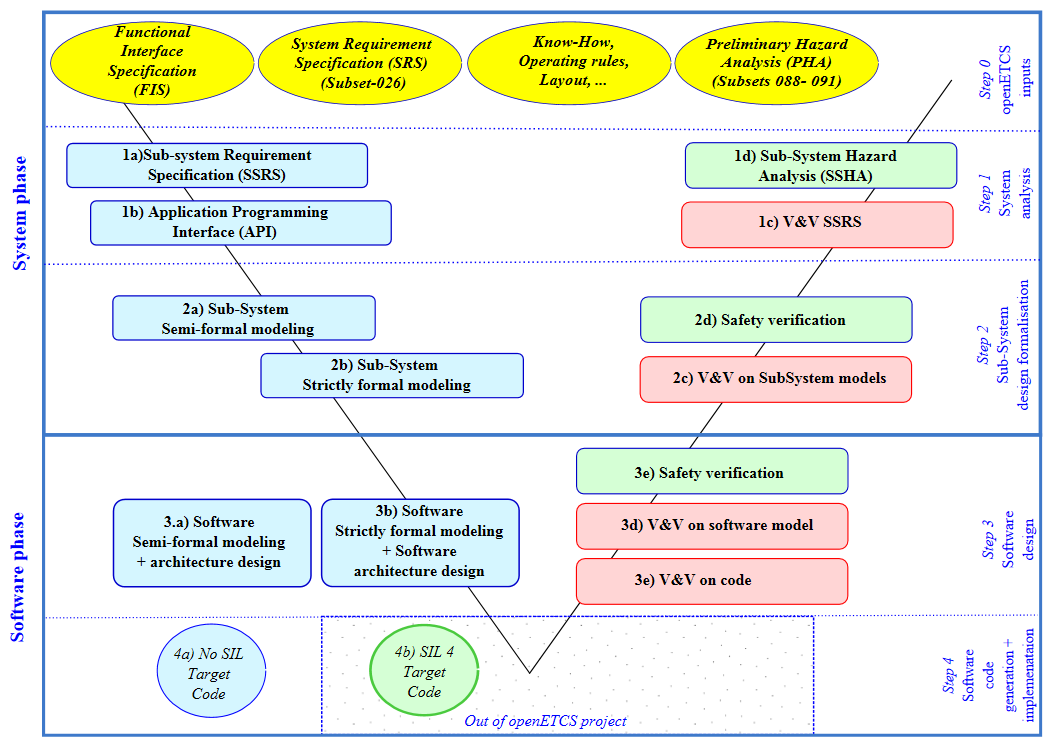
\includegraphics[width=.9\textwidth]{images/ProcessOpenETCS-BeM.png}
  \caption{openETCS Process (rough view)}
  \label{fig:openETCSProcess}
\end{figure}

According figure \ref{fig:openETCSProcess}, for which activities is the mean or tool suitable (see also \citep{D4.1} section 5.1.2 for more details)\footnote{DAS2V : Design Artifact Subject to Verification and Validation, see \citep{D4.1}} ?


\begin{tabular}{|l | c | c | c | c|}
\hline
& \textcolor{green}{Author} & \textcolor{blue}{Assessor 1} & \textcolor{magenta}{Assessor 2} & Total \\
\hline 
1c SSRS Verification & & & &  \\
\hline
1c SSRS Validation & & & &  \\
\hline
2c SFM Verification & & & &  \\
\hline
2c SFM Validation & & & &  \\
\hline
3d SW-SFM Verification & & & &  \\
\hline
3d SW-SFM Validation & & & &  \\
\hline
3d SW-FFM Verification & & & &  \\
\hline
3d SW-FFM Validation & & & &  \\
\hline
3e Code Verification & & & &  \\
\hline
3e Code Validation & & & &  \\
\hline
DAS2V Verification & & & &  \\
\hline
DAS2V Validation & & & &  \\
\hline
Automatic model transformation verification & & & &  \\
\hline
Automatic code generation verification & & & &  \\
\hline
\end{tabular}


\section{Properties}

Which kind of properties or elements are verified or validated by the mean or tool (see also \citep{D4.1} section 4)  ?



\begin{tabular}{|l | c | c | c | c|}
\hline
& \textcolor{green}{Author} & \textcolor{blue}{Assessor 1} & \textcolor{magenta}{Assessor 2} & Total \\
\hline 
Functionalities of the system and sub-system & & & &  \\
\hline
System and sub-system architecture & & & &  \\
\hline
External and internal interfaces of sub-system & & & &  \\
\hline
Software components & & & &  \\
\hline
Performance constraints & & & &  \\
\hline
Safety objectives & & & &  \\
\hline
Functional properties & & & &  \\
\hline
Safety properties & & & &  \\
\hline
\end{tabular}



\section{Verification methods and tools}

Which kind of methods is proposed (see also \citep{D4.1} section 5.3) ?



\begin{tabular}{|l | c | c | c | c|}
\hline
& \textcolor{green}{Author} & \textcolor{blue}{Assessor 1} & \textcolor{magenta}{Assessor 2} & Total \\
\hline 
Reviews & & & &  \\
\hline
Inspections & & & &  \\
\hline
Software Architecture Analysis Method & & & &  \\
\hline
Architecture Tradeoff Analysis Method & & & &  \\
\hline
Model-Based System Integration Testing & & & &  \\
\hline
Model-Based Testing of Generated High-Level Code & & & &  \\
\hline
Abstract Interpretation & & & &  \\
\hline
Deductive Verification & & & &  \\
\hline
Model Checking & & & &  \\
\hline
Correct by Construction Formal Methods & & & &  \\
\hline
Verification with Formal Methods & & & &  \\
\hline
Simulation-based & & & &  \\
\hline
\end{tabular}

\section{Validation means and tools}

The following list of criteria focuss on means and tools to support validation activities, according WP2  requirements :

\begin{tabular}{|l | c | c | c | c|}
\hline
& \textcolor{green}{Author} & \textcolor{blue}{Assessor 1} & \textcolor{magenta}{Assessor 2} & Total \\
\hline 
Simulation-based & & & &  \\
\hline
Step-by-step simulation (D2.6-01-036) & & & &  \\
\hline
Environment emulation (D2.6-01-037 and D2.6-02-080) & & & &  \\
\hline
Time-based test case (D2.6-02-081) & & & &  \\
\hline
Test cases writing (D2.6-01-038) & & & &  \\
\hline
Test cases execution (D2.6-01-038) & & & &  \\
\hline
Test cases storage (D2.6-01-038) & & & &  \\
\hline
Version management of test cases (D2.6-02-082) & & & &  \\
\hline
Test generation from independant test model (D2.6-02-083) & & & &  \\
\hline
Test sequences writing (D2.6-02-084) & & & &  \\
\hline
Test sequences execution (D2.6-02-084) & & & &  \\
\hline
Test sequences storage (D2.6-02-084) & & & &  \\
\hline
\end{tabular}

\section{VnV artifacts}


Concerning the artifacts used or produced by the mean or tool, please to detail:

\paragraph{Input}
    Which is the list of the input artifacts for the mean or tools ?
    
    
\paragraph{Output}
    Which is the list of the output artifacts for the mean or tools ?
    
\paragraph{Syntax}
    Which are the reference documents which give a description of the artifacts syntax  ?
    
\paragraph{Semantic}
    Which are the reference documents which give a description of the artifacts semantic  ?


\paragraph{Integration}
    How these artifacts can be integrated with the elements of the toolchain (language, mangement,...) ?


\section{Detailled Criterias for VnV}

Please  fill only the section concerning the proposed mean or tool, other section can be skipped (see issue \url{https://github.com/openETCS/toolchain/issues/180} for details and discussions)



\subsection{System Modelling simulation}	

\begin{tabular}{|l | c | c | c | c|}
\hline
& \textcolor{green}{Author} & \textcolor{blue}{Assessor 1} & \textcolor{magenta}{Assessor 2} & Total \\
\hline 
User Scenario Modelling & & & &  \\
\hline
Test Case Modelling & & & &  \\
\hline
Test Sequence Modelling & & & &  \\
\hline
\end{tabular}
	
\subsection{System Model Verification}	


\begin{tabular}{|l | c | c | c | c|}
\hline
& \textcolor{green}{Author} & \textcolor{blue}{Assessor 1} & \textcolor{magenta}{Assessor 2} & Total \\
\hline 
Input/ Output checking & & & &  \\
\hline
System Behavior Simulation (Mathematical) & & & &  \\
\hline
System Behavior Simulation (Animated) & & & &  \\
\hline
\end{tabular}


\subsection{Software Model Verification	}


\begin{tabular}{|l | c | c | c | c|}
\hline
& \textcolor{green}{Author} & \textcolor{blue}{Assessor 1} & \textcolor{magenta}{Assessor 2} & Total \\
\hline 
Static Model Verification & & & &  \\
\hline
Property Proofing & & & &  \\
\hline
Dynamic Testing & & & &  \\
\hline
Automatic Test Generation & & & &  \\
\hline
Input/ Output checking & & & &  \\
\hline
Software Behaviour Simulation (Mathematical) & & & &  \\
\hline
Software Behaviour Simulation (Animated) & & & &  \\
\hline
\end{tabular}


\subsection{Source Code}


\begin{tabular}{|l | c | c | c | c|}
\hline
& \textcolor{green}{Author} & \textcolor{blue}{Assessor 1} & \textcolor{magenta}{Assessor 2} & Total \\
\hline 
Traceability to Model & & & &  \\
\hline
\end{tabular}


\subsection{Code Verification	}


\begin{tabular}{|l | c | c | c | c|}
\hline
& \textcolor{green}{Author} & \textcolor{blue}{Assessor 1} & \textcolor{magenta}{Assessor 2} & Total \\
\hline 
Formal Proof & & & &  \\
\hline
Programming by contract & & & &  \\
\hline
Static Analysis & & & &  \\
\hline
Dynamic Analysis & & & &  \\
\hline
Dynamic Testing & & & &  \\
\hline
Automatic Test Generation & & & &  \\
\hline
Performance Testing & & & &  \\
\hline
Interface Testing & & & &  \\
\hline
\end{tabular}

	
\subsection{Validation System/Software/Code/ Validation	}


\begin{tabular}{|l | c | c | c | c|}
\hline
& \textcolor{green}{Author} & \textcolor{blue}{Assessor 1} & \textcolor{magenta}{Assessor 2} & Total \\
\hline 
Test Coverage & & & &  \\
\hline
Use Case Validation of Model & & & &  \\
\hline
Functional or Black-box Testing & & & &  \\
\hline
User Scenario Testing & & & &  \\
\hline
Traceability & & & &  \\
\hline
Schedulability Analyzer / UseCase Check all & & & &  \\
\hline
Schedulability Analyzer / UseCase Check single mode & & & &  \\
\hline

\end{tabular}



\section{Other comments}



\begin{comment}
This section is available for the author or the assessors to  complete the description and criteria.
\end{comment}




\chapter{Diversity}
\label{sec:diversity}

\section{Instructions}

\begin{description}
\item[\textcolor{green}{Author}] Author of the approaches description  \todo{Name -  Company}
\item[\textcolor{blue}{Assessor 1}] First assessor of the approaches \todo{Name - Company}
\item[\textcolor{magenta}{Assessor 2}] Second assessor of the approaches \todo{Name - Company}
\end{description}

In the sequel, main text is under the responsibilities of the author.

\begin{author_comment}
Author can add comments using this format at any place.
\end{author_comment}

\begin{assessor1}
First assessor can add comments using this format at any place.
\end{assessor1}

\begin{assessor2}
Second assessor can add comments using this format at any place.
\end{assessor2}

When a note is required, please follow this list (inspired from Technology Readiness Level, see \url{http://en.wikipedia.org/wiki/Technology\_readiness\_level}) :

\begin{description}
\item[0] not recommended / rejected / no integration possible or valuable / not adapted for this topic / not available for this topic
\item[1] weakly recommended / adapted after major improvements / weakly rejected / concept of integration roughly defined / adapted after major improvements / available after major developments
\item[2] recommended / adapted (with light improvements if necessary)  weakly accepted / integration prototyped or defined in details / adapted after small improvements / available after small developments or tests
\item[3] highly recommended / well adapted / strongly accepted / integration done and tested / well adapted to the purpose / available and suitable for the purpose All the notes can be commented under each table.
\item[*] difficult to evaluate with a note (please add a comment under the table)
\end{description}


All the notes can be commented under each table.

This section defines the criteria for the means and tools dedicated to verification and validation activities, in the WP4 workpackage. 

Criteria of this section are defined according \citep{D4.1}.

\section{Presentation}

This section gives a quick presentation of the approach and the tool.

\begin{description}
\item[Name] \todo{Name of the approach and the tool}
\item[Web site] \todo{if available, how to  find information}
\item[Licence] \todo{Kind of licence}
\end{description}

\paragraph{Abstract} Short abstract on the approach and tool (10 lines max)

\paragraph{Publications} Short list of publications on the approach (5 max)


\section{Common criteria on secondary means and tools}
\label{common}
This section discusses the common criteria of the means and tools according to the project requirements on tools and the results of T7.1.

\subsection{Project and WP2 requirements}

The objectives of this list of criteria is to check if the proposed means and tools meet the main criteria of the project: open-source approaches, usability, modularity, coverage of the objectives,...

According WP2 requirements, give a note for characteristics of the use of the tool (from 0 to 3) :

\begin{tabular}{|l | c | c | c | c|}
\hline
& \textcolor{green}{Author} & \textcolor{blue}{Assessor 1} & \textcolor{magenta}{Assessor 2} & Total \\
\hline 
Open Source (D2.6-02-074) & & & &  \\
\hline 
Portability to operating systems (D2.6-02-075) & & & &  \\
\hline
Cooperation of tools (D2.6-02-076) & & & &  \\
\hline
Robustness (D2.6-02-078) & & & & \\
\hline
Modularity (D2.6-02-078.1) & & & & \\
\hline
Documentation management (D2.6-02-078.02) & & & & \\
\hline
Distributed software development (D2.6-02-078.03)  & & & & \\
\hline
Simultaneous multi-users (D2.6-02-078.04)   & & & & \\
\hline
Issue tracking (D2.6-02-078.05) & & & & \\
\hline
Differences between models (D2.6-02-078.06) & & & & \\
\hline
Version management (D2.6-02-078.07) & & & & \\
\hline
Concurrent version development (D2.6-02-078.08) & & & & \\
\hline
Model-based version control (D2.6-02-078.09) & & & & \\
\hline
Role traceability (D2.6-02-078.10) & & & & \\
\hline
Safety version traceability (D2.6-02-078.11) & & & & \\
\hline
Model traceability (D2.6-02-079) & & & & \\
\hline
Tool chain integration & & & & \\
\hline
Scalability & & & & \\
\hline
User Friendliness & & & & \\
\hline
\end{tabular}



\subsection{Qualification}

This section discusses how the tool can be classified according EN50128 requirements (D2.6-02-085). Some qualification shall be mandatory  if the tool is involved to design a SIL4 software.


\begin{tabular}{|l | c | c | c | c|}
\hline
& \textcolor{green}{Author} & \textcolor{blue}{Assessor 1} & \textcolor{magenta}{Assessor 2} & Total \\
\hline 
Tool manual (D.2.6-01-42.02) & & & &  \\
\hline
Proof of correctness (D.2.6-01-42.03)   & & & & \\
\hline
Existing industrial  usage  & & & & \\
\hline
Model verification & & & & \\
\hline
Test generation & & & & \\
\hline
Simulation, execution, debugging & & & & \\
\hline
Formal proof & & & & \\
\hline
\end{tabular}


Which level of tool qualification has been reached or will be reached within the next year ?

Score :
\begin{description}
\item[3] already qualified for this level
\item[2] qualification possible to this level, but some elements shall be provided
\item[0] qualification not recommended for this level
\end{description}


\begin{tabular}{|l | c | c | c | c|}
\hline
& \textcolor{green}{Author} & \textcolor{blue}{Assessor 1} & \textcolor{magenta}{Assessor 2} & Total \\
\hline 
class T1 & & & &  \\
\hline
class T2   & & & & \\
\hline
class T3  & & & & \\
\hline
\end{tabular}

\paragraph{Other elements for tool certification}


\subsection{Complementarity with primary toolchain}

The objectives of this list of criteria is to check if the proposed means and tools can be easily integrated to the primary toolchain.

\subsubsection{Language}


According to the decisions and the propositions of T7.1, how the mean and approach can be adapted to or can complete the chosen language and methods:

\begin{tabular}{|l | c | c | c | c|}
\hline
& \textcolor{green}{Author} & \textcolor{blue}{Assessor 1} & \textcolor{magenta}{Assessor 2} & Total \\
\hline 
SysML  & & & & \\
\hline
Scade method & & & & \\
\hline
EFS language & & & & \\
\hline
B Method & & & & \\
\hline
C language & & & & \\
\hline
\end{tabular}

\paragraph{SysML}
How the means or tools can complete SysML ?


\paragraph{Scade, EFS, Classical B}
How the means or tools can complete the current proposals for formal modeling language ?

\paragraph{C language}
How the means or tools can complete or be adapted to SIL4 software in C language ?

\subsubsection{Tools and platforms}

According to the decisions and the propositions of T7.1, how the mean and approach can be integrated to or can complete the chosen tools and platforms:

\begin{tabular}{|l | c | c | c | c|}
\hline
& \textcolor{green}{Author} & \textcolor{blue}{Assessor 1} & \textcolor{magenta}{Assessor 2} & Total \\
\hline 
Eclipse & & & &  \\
\hline
Papyrus  & & & & \\
\hline
Scade & & & & \\
\hline
EFS tools & & & & \\
\hline
B tools & & & & \\
\hline
\end{tabular}


\paragraph{Eclipse}
How the means or tools can be integrated to the Eclipse platform ?

\paragraph{Papyrus}
How the means or tools can complete  Papyrus ?


\paragraph{Scade, EFS, Classical B}
How the means or tools can complete the current proposals for formal modeling tools ?





\section{VnV Activities}

The VnV activities are described in details in the verification and Validation Plan  \citep{D4.1}.

\begin{figure}[htb]
  \centering
  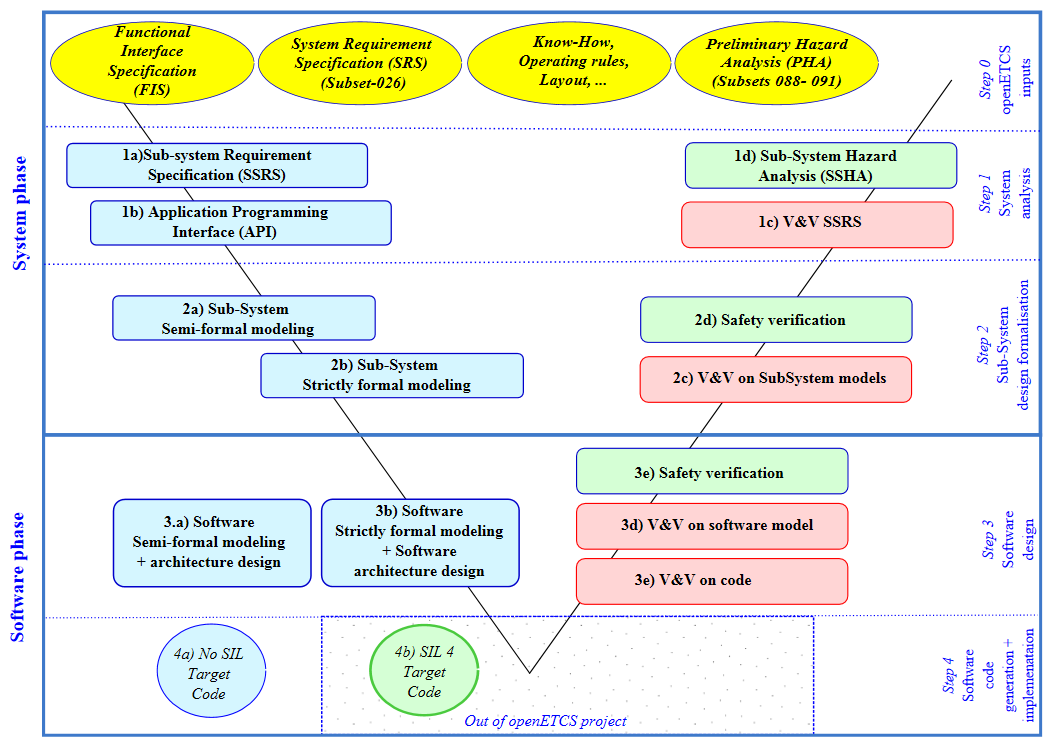
\includegraphics[width=.9\textwidth]{images/ProcessOpenETCS-BeM.png}
  \caption{openETCS Process (rough view)}
  \label{fig:openETCSProcess}
\end{figure}

According figure \ref{fig:openETCSProcess}, for which activities is the mean or tool suitable (see also \citep{D4.1} section 5.1.2 for more details)\footnote{DAS2V : Design Artifact Subject to Verification and Validation, see \citep{D4.1}} ?


\begin{tabular}{|l | c | c | c | c|}
\hline
& \textcolor{green}{Author} & \textcolor{blue}{Assessor 1} & \textcolor{magenta}{Assessor 2} & Total \\
\hline 
1c SSRS Verification & & & &  \\
\hline
1c SSRS Validation & & & &  \\
\hline
2c SFM Verification & & & &  \\
\hline
2c SFM Validation & & & &  \\
\hline
3d SW-SFM Verification & & & &  \\
\hline
3d SW-SFM Validation & & & &  \\
\hline
3d SW-FFM Verification & & & &  \\
\hline
3d SW-FFM Validation & & & &  \\
\hline
3e Code Verification & & & &  \\
\hline
3e Code Validation & & & &  \\
\hline
DAS2V Verification & & & &  \\
\hline
DAS2V Validation & & & &  \\
\hline
Automatic model transformation verification & & & &  \\
\hline
Automatic code generation verification & & & &  \\
\hline
\end{tabular}


\section{Properties}

Which kind of properties or elements are verified or validated by the mean or tool (see also \citep{D4.1} section 4)  ?



\begin{tabular}{|l | c | c | c | c|}
\hline
& \textcolor{green}{Author} & \textcolor{blue}{Assessor 1} & \textcolor{magenta}{Assessor 2} & Total \\
\hline 
Functionalities of the system and sub-system & & & &  \\
\hline
System and sub-system architecture & & & &  \\
\hline
External and internal interfaces of sub-system & & & &  \\
\hline
Software components & & & &  \\
\hline
Performance constraints & & & &  \\
\hline
Safety objectives & & & &  \\
\hline
Functional properties & & & &  \\
\hline
Safety properties & & & &  \\
\hline
\end{tabular}



\section{Verification methods and tools}

Which kind of methods is proposed (see also \citep{D4.1} section 5.3) ?



\begin{tabular}{|l | c | c | c | c|}
\hline
& \textcolor{green}{Author} & \textcolor{blue}{Assessor 1} & \textcolor{magenta}{Assessor 2} & Total \\
\hline 
Reviews & & & &  \\
\hline
Inspections & & & &  \\
\hline
Software Architecture Analysis Method & & & &  \\
\hline
Architecture Tradeoff Analysis Method & & & &  \\
\hline
Model-Based System Integration Testing & & & &  \\
\hline
Model-Based Testing of Generated High-Level Code & & & &  \\
\hline
Abstract Interpretation & & & &  \\
\hline
Deductive Verification & & & &  \\
\hline
Model Checking & & & &  \\
\hline
Correct by Construction Formal Methods & & & &  \\
\hline
Verification with Formal Methods & & & &  \\
\hline
Simulation-based & & & &  \\
\hline
\end{tabular}

\section{Validation means and tools}

The following list of criteria focuss on means and tools to support validation activities, according WP2  requirements :

\begin{tabular}{|l | c | c | c | c|}
\hline
& \textcolor{green}{Author} & \textcolor{blue}{Assessor 1} & \textcolor{magenta}{Assessor 2} & Total \\
\hline 
Simulation-based & & & &  \\
\hline
Step-by-step simulation (D2.6-01-036) & & & &  \\
\hline
Environment emulation (D2.6-01-037 and D2.6-02-080) & & & &  \\
\hline
Time-based test case (D2.6-02-081) & & & &  \\
\hline
Test cases writing (D2.6-01-038) & & & &  \\
\hline
Test cases execution (D2.6-01-038) & & & &  \\
\hline
Test cases storage (D2.6-01-038) & & & &  \\
\hline
Version management of test cases (D2.6-02-082) & & & &  \\
\hline
Test generation from independant test model (D2.6-02-083) & & & &  \\
\hline
Test sequences writing (D2.6-02-084) & & & &  \\
\hline
Test sequences execution (D2.6-02-084) & & & &  \\
\hline
Test sequences storage (D2.6-02-084) & & & &  \\
\hline
\end{tabular}

\section{VnV artifacts}


Concerning the artifacts used or produced by the mean or tool, please to detail:

\paragraph{Input}
    Which is the list of the input artifacts for the mean or tools ?
    
    
\paragraph{Output}
    Which is the list of the output artifacts for the mean or tools ?
    
\paragraph{Syntax}
    Which are the reference documents which give a description of the artifacts syntax  ?
    
\paragraph{Semantic}
    Which are the reference documents which give a description of the artifacts semantic  ?


\paragraph{Integration}
    How these artifacts can be integrated with the elements of the toolchain (language, mangement,...) ?


\section{Detailled Criterias for VnV}

Please  fill only the section concerning the proposed mean or tool, other section can be skipped (see issue \url{https://github.com/openETCS/toolchain/issues/180} for details and discussions)



\subsection{System Modelling simulation}	

\begin{tabular}{|l | c | c | c | c|}
\hline
& \textcolor{green}{Author} & \textcolor{blue}{Assessor 1} & \textcolor{magenta}{Assessor 2} & Total \\
\hline 
User Scenario Modelling & & & &  \\
\hline
Test Case Modelling & & & &  \\
\hline
Test Sequence Modelling & & & &  \\
\hline
\end{tabular}
	
\subsection{System Model Verification}	


\begin{tabular}{|l | c | c | c | c|}
\hline
& \textcolor{green}{Author} & \textcolor{blue}{Assessor 1} & \textcolor{magenta}{Assessor 2} & Total \\
\hline 
Input/ Output checking & & & &  \\
\hline
System Behavior Simulation (Mathematical) & & & &  \\
\hline
System Behavior Simulation (Animated) & & & &  \\
\hline
\end{tabular}


\subsection{Software Model Verification	}


\begin{tabular}{|l | c | c | c | c|}
\hline
& \textcolor{green}{Author} & \textcolor{blue}{Assessor 1} & \textcolor{magenta}{Assessor 2} & Total \\
\hline 
Static Model Verification & & & &  \\
\hline
Property Proofing & & & &  \\
\hline
Dynamic Testing & & & &  \\
\hline
Automatic Test Generation & & & &  \\
\hline
Input/ Output checking & & & &  \\
\hline
Software Behaviour Simulation (Mathematical) & & & &  \\
\hline
Software Behaviour Simulation (Animated) & & & &  \\
\hline
\end{tabular}


\subsection{Source Code}


\begin{tabular}{|l | c | c | c | c|}
\hline
& \textcolor{green}{Author} & \textcolor{blue}{Assessor 1} & \textcolor{magenta}{Assessor 2} & Total \\
\hline 
Traceability to Model & & & &  \\
\hline
\end{tabular}


\subsection{Code Verification	}


\begin{tabular}{|l | c | c | c | c|}
\hline
& \textcolor{green}{Author} & \textcolor{blue}{Assessor 1} & \textcolor{magenta}{Assessor 2} & Total \\
\hline 
Formal Proof & & & &  \\
\hline
Programming by contract & & & &  \\
\hline
Static Analysis & & & &  \\
\hline
Dynamic Analysis & & & &  \\
\hline
Dynamic Testing & & & &  \\
\hline
Automatic Test Generation & & & &  \\
\hline
Performance Testing & & & &  \\
\hline
Interface Testing & & & &  \\
\hline
\end{tabular}

	
\subsection{Validation System/Software/Code/ Validation	}


\begin{tabular}{|l | c | c | c | c|}
\hline
& \textcolor{green}{Author} & \textcolor{blue}{Assessor 1} & \textcolor{magenta}{Assessor 2} & Total \\
\hline 
Test Coverage & & & &  \\
\hline
Use Case Validation of Model & & & &  \\
\hline
Functional or Black-box Testing & & & &  \\
\hline
User Scenario Testing & & & &  \\
\hline
Traceability & & & &  \\
\hline
Schedulability Analyzer / UseCase Check all & & & &  \\
\hline
Schedulability Analyzer / UseCase Check single mode & & & &  \\
\hline

\end{tabular}



\section{Other comments}



\begin{comment}
This section is available for the author or the assessors to  complete the description and criteria.
\end{comment}






%%%%%%%%%%%%%%%%%%%%%%%%%%%

%% Bibliography

\bibliographystyle{plain}
\bibliography{wp7_bibliography}



%===================================================
%Do NOT change anything below this line

\end{document}
